\documentclass[a4paper, 11pt, svgnames]{report}
\usepackage[margin=3cm]{geometry}
\usepackage[T1]{fontenc}
\usepackage[utf8]{inputenc}
\usepackage[french]{babel}
\usepackage{hyperref}
\usepackage[toc,acronym,nopostdot]{glossaries}
\usepackage{graphicx}
\usepackage{float}
\usepackage{minted}
\usepackage{mathtools}
\usepackage[toc, page]{appendix}
\usepackage{subcaption}
\usepackage{rotating}
\usepackage{pst-circ}

\usepackage{tikz}
\usetikzlibrary{decorations.text, arrows, arrows.spaced ,automata, snakes, circuits.logic.US, calc, shapes.geometric}

\tikzstyle{block} = [draw]
\tikzstyle{asyncblock} = [draw]


\pagestyle{empty}
\makeatletter

\tikzset{add font/.code={\expandafter\def\expandafter\tikz@textfont\expandafter{\tikz@textfont#1}}}
\tikzset{port labels/.style={font=\sffamily\scriptsize}}

%
% Default style for components
%

\tikzset{every srr node/.style={draw,minimum width=2cm,minimum height=2cm,inner sep=1mm,outer sep=0pt,cap=round,add font=\sffamily}}
\tikzset{every dff node/.style={draw,minimum width=1cm,minimum height=1.5cm,inner sep=1mm,outer sep=0pt,cap=round,add font=\sffamily}}
\tikzset{every syndrome node/.style={draw,minimum width=5cm,minimum height=2cm,inner sep=1mm,outer sep=0pt,cap=round,add font=\sffamily}}
\tikzset{every utsyndrome node/.style={draw,minimum width=5cm,minimum height=2cm,inner sep=1mm,outer sep=0pt,cap=round,add font=\sffamily}}
\tikzset{every ucsyndrome node/.style={draw,minimum width=5cm,minimum height=2cm,inner sep=1mm,outer sep=0pt,cap=round,add font=\sffamily}}


%
% Shift right register
%

\pgfdeclareshape{srr}{
    % The 'minimum width' and 'minimum height' keys, not the content, determine
    % the size
    \savedanchor\northeast{%
        \pgfmathsetlength\pgf@x{\pgfshapeminwidth}%
        \pgfmathsetlength\pgf@y{\pgfshapeminheight}%
        \pgf@x=0.5\pgf@x
        \pgf@y=0.5\pgf@y
    }
    % This is redundant, but makes some things easier:
    \savedanchor\southwest{%
        \pgfmathsetlength\pgf@x{\pgfshapeminwidth}%
        \pgfmathsetlength\pgf@y{\pgfshapeminheight}%
        \pgf@x=-0.5\pgf@x
        \pgf@y=-0.5\pgf@y
    }
    % Inherit from rectangle
    \inheritanchorborder[from=rectangle]

    % Define same anchor a normal rectangle has
    \anchor{center}{\pgfpointorigin}
    \anchor{north}{\northeast \pgf@x=0pt}
    \anchor{east}{\northeast \pgf@y=0pt}
    \anchor{south}{\southwest \pgf@x=0pt}
    \anchor{west}{\southwest \pgf@y=0pt}
    \anchor{north east}{\northeast}
    \anchor{north west}{\northeast \pgf@x=-\pgf@x}
    \anchor{south west}{\southwest}
    \anchor{south east}{\southwest \pgf@x=-\pgf@x}
    \anchor{text}{
        \pgfpointorigin
        \advance\pgf@x by -.5\wd\pgfnodeparttextbox%
        \advance\pgf@y by -.5\ht\pgfnodeparttextbox%
        \advance\pgf@y by +.5\dp\pgfnodeparttextbox%
    }

    % Define anchors for signal ports
    \anchor{Din}{
        \pgf@process{\northeast}%
        \pgf@x=-1\pgf@x%
        \pgf@y=0.75\pgf@y%
    }
    \anchor{Ld}{
        \pgf@process{\northeast}%
        \pgf@x=-1\pgf@x%
        \pgf@y=0.375\pgf@y%
    }
    \anchor{Shift}{
        \pgf@process{\northeast}%
        \pgf@x=-1\pgf@x%
        \pgf@y=0\pgf@y%
    }
    \anchor{CLK}{
        \pgf@process{\northeast}%
        \pgf@x=-1\pgf@x%
        \pgf@y=-.75\pgf@y%
    }
    \anchor{Dout}{
        \pgf@process{\northeast}%
        \pgf@y=0\pgf@y%
    }

    % Draw the rectangle box and the port labels
    \backgroundpath{
        % Rectangle box
        \pgfpathrectanglecorners{\southwest}{\northeast}
        % Angle (>) for clock input
        \pgf@anchor@srr@CLK
        \pgf@xa=\pgf@x \pgf@ya=\pgf@y
        \pgf@xb=\pgf@x \pgf@yb=\pgf@y
        \pgf@xc=\pgf@x \pgf@yc=\pgf@y
        \pgfmathsetlength\pgf@x{1ex} % size depends on font size
        \advance\pgf@ya by \pgf@x
        \advance\pgf@xb by \pgf@x
        \advance\pgf@yc by -\pgf@x
        \pgfpathmoveto{\pgfpoint{\pgf@xa}{\pgf@ya}}
        \pgfpathlineto{\pgfpoint{\pgf@xb}{\pgf@yb}}
        \pgfpathlineto{\pgfpoint{\pgf@xc}{\pgf@yc}}
        \pgfclosepath

        % Draw port labels
        \begingroup
        \tikzset{port labels} % Use font from this style
        \tikz@textfont
        \tikz@textfont

        \pgf@anchor@srr@Din
        \pgftext[left,base,at={\pgfpoint{\pgf@x}{\pgf@y}},x=\pgfshapeinnerxsep]{\raisebox{-0.75ex}{Din}}

        \pgf@anchor@srr@CLK
        \pgftext[left,base,at={\pgfpoint{\pgf@x}{\pgf@y}},x=\pgfshapeinnerxsep]{\raisebox{-0.75ex}{}}

        \pgf@anchor@srr@Dout
        \pgftext[right,base,at={\pgfpoint{\pgf@x}{\pgf@y}},x=-\pgfshapeinnerxsep]{\raisebox{-0.75ex}{Dout}}

        \pgf@anchor@srr@Ld
        \pgftext[left,base,at={\pgfpoint{\pgf@x}{\pgf@y}},x=\pgfshapeinnerxsep]{\raisebox{-0.75ex}{Ld}}

        \pgf@anchor@srr@Shift
        \pgftext[left,base,at={\pgfpoint{\pgf@x}{\pgf@y}},x=\pgfshapeinnerxsep]{\raisebox{-0.75ex}{Shift}}

        \endgroup
    }
}

%
% Data Flip Flip (DFF) shape
%

\pgfdeclareshape{dff}{
  % The 'minimum width' and 'minimum height' keys, not the content, determine
  % the size
    \savedanchor\northeast{%
        \pgfmathsetlength\pgf@x{\pgfshapeminwidth}%
        \pgfmathsetlength\pgf@y{\pgfshapeminheight}%
        \pgf@x=0.5\pgf@x
        \pgf@y=0.5\pgf@y
    }
  % This is redundant, but makes some things easier:
    \savedanchor\southwest{%
        \pgfmathsetlength\pgf@x{\pgfshapeminwidth}%
        \pgfmathsetlength\pgf@y{\pgfshapeminheight}%
        \pgf@x=-0.5\pgf@x
        \pgf@y=-0.5\pgf@y
    }
    % Inherit from rectangle
    \inheritanchorborder[from=rectangle]

    % Define same anchor a normal rectangle has
    \anchor{center}{\pgfpointorigin}
    \anchor{north}{\northeast \pgf@x=0pt}
    \anchor{east}{\northeast \pgf@y=0pt}
    \anchor{south}{\southwest \pgf@x=0pt}
    \anchor{west}{\southwest \pgf@y=0pt}
    \anchor{north east}{\northeast}
    \anchor{north west}{\northeast \pgf@x=-\pgf@x}
    \anchor{south west}{\southwest}
    \anchor{south east}{\southwest \pgf@x=-\pgf@x}
    \anchor{text}{
        \pgfpointorigin
        \advance\pgf@x by -.5\wd\pgfnodeparttextbox%
        \advance\pgf@y by -.5\ht\pgfnodeparttextbox%
        \advance\pgf@y by +.5\dp\pgfnodeparttextbox%
    }

    % Define anchors for signal ports
    \anchor{D}{
        \pgf@process{\northeast}%
        \pgf@x=-1\pgf@x%
        \pgf@y=.5\pgf@y%
    }
    \anchor{CLK}{
        \pgf@process{\northeast}%
        \pgf@x=-1\pgf@x%
        \pgf@y=-.5\pgf@y%
    }
    \anchor{Q}{
        \pgf@process{\northeast}%
        \pgf@y=.5\pgf@y%
    }
    \anchor{Qn}{
        \pgf@process{\northeast}%
        \pgf@y=-.5\pgf@y%
    }

    \anchor{R}{
        \pgf@process{\northeast}%
        \pgf@x=0pt%
    }
    \anchor{S}{
        \pgf@process{\northeast}%
        \pgf@x=0pt%
        \pgf@y=-\pgf@y%
    }

    % Draw the rectangle box and the port labels
    \backgroundpath{
        % Rectangle box
        \pgfpathrectanglecorners{\southwest}{\northeast}
        % Angle (>) for clock input
        \pgf@anchor@dff@CLK
        \pgf@xa=\pgf@x \pgf@ya=\pgf@y
        \pgf@xb=\pgf@x \pgf@yb=\pgf@y
        \pgf@xc=\pgf@x \pgf@yc=\pgf@y
        \pgfmathsetlength\pgf@x{1ex} % size depends on font size
        \advance\pgf@ya by \pgf@x
        \advance\pgf@xb by \pgf@x
        \advance\pgf@yc by -\pgf@x
        \pgfpathmoveto{\pgfpoint{\pgf@xa}{\pgf@ya}}
        \pgfpathlineto{\pgfpoint{\pgf@xb}{\pgf@yb}}
        \pgfpathlineto{\pgfpoint{\pgf@xc}{\pgf@yc}}
        \pgfclosepath

        % Draw port labels
        \begingroup
        \tikzset{port labels} % Use font from this style
        \tikz@textfont

        \pgf@anchor@dff@D
        \pgftext[left,base,at={\pgfpoint{\pgf@x}{\pgf@y}},x=\pgfshapeinnerxsep]{\raisebox{-0.75ex}{D}}

        \pgf@anchor@dff@Q
        \pgftext[right,base,at={\pgfpoint{\pgf@x}{\pgf@y}},x=-\pgfshapeinnerxsep]{\raisebox{-.75ex}{Q}}

        \pgf@anchor@dff@Qn
        \pgftext[right,base,at={\pgfpoint{\pgf@x}{\pgf@y}},x=-\pgfshapeinnerxsep]{\raisebox{-.75ex}{$\overline{\mbox{Q}}$}}

        \pgf@anchor@dff@R
        \pgftext[top,at={\pgfpoint{\pgf@x}{\pgf@y}},y=-\pgfshapeinnerysep]{R}

        \pgf@anchor@dff@S
        \pgftext[bottom,at={\pgfpoint{\pgf@x}{\pgf@y}},y=\pgfshapeinnerysep]{S}

        \endgroup
    }
}


%
% External syndrome block
%

\pgfdeclareshape{syndrome}{
  % The 'minimum width' and 'minimum height' keys, not the content, determine
  % the size
    \savedanchor\northeast{%
        \pgfmathsetlength\pgf@x{\pgfshapeminwidth}%
        \pgfmathsetlength\pgf@y{\pgfshapeminheight}%
        \pgf@x=0.5\pgf@x
        \pgf@y=0.5\pgf@y
    }
  % This is redundant, but makes some things easier:
    \savedanchor\southwest{%
        \pgfmathsetlength\pgf@x{\pgfshapeminwidth}%
        \pgfmathsetlength\pgf@y{\pgfshapeminheight}%
        \pgf@x=-0.5\pgf@x
        \pgf@y=-0.5\pgf@y
    }
    % Inherit from rectangle
    \inheritanchorborder[from=rectangle]

    % Define same anchor a normal rectangle has
    \anchor{center}{\pgfpointorigin}
    \anchor{north}{\northeast \pgf@x=0pt}
    \anchor{east}{\northeast \pgf@y=0pt}
    \anchor{south}{\southwest \pgf@x=0pt}
    \anchor{west}{\southwest \pgf@y=0pt}
    \anchor{north east}{\northeast}
    \anchor{north west}{\northeast \pgf@x=-\pgf@x}
    \anchor{south west}{\southwest}
    \anchor{south east}{\southwest \pgf@x=-\pgf@x}
    \anchor{text}{
        \pgfpointorigin
        \advance\pgf@x by -.5\wd\pgfnodeparttextbox%
        \advance\pgf@y by -.5\ht\pgfnodeparttextbox%
        \advance\pgf@y by +.5\dp\pgfnodeparttextbox%
    }

    % Define anchors for signal ports
    \anchor{Data}{
        \pgf@process{\northeast}%
        \pgf@x=-1\pgf@x%
        \pgf@y=.75\pgf@y%
    }
    \anchor{Start}{
        \pgf@process{\northeast}%
        \pgf@x=-1\pgf@x%
        \pgf@y=.25\pgf@y%
    }
    \anchor{Reset}{
        \pgf@process{\northeast}%
        \pgf@x=-1\pgf@x%
        \pgf@y=-.25\pgf@y%
    }
    \anchor{CLK}{
        \pgf@process{\northeast}%
        \pgf@x=-1\pgf@x%
        \pgf@y=-.75\pgf@y%
    }

    \anchor{Syndrome}{
        \pgf@process{\northeast}%
        \pgf@y=.5\pgf@y%
    }
    \anchor{End}{
        \pgf@process{\northeast}%
        \pgf@y=-.5\pgf@y%
    }

    % Draw the rectangle box and the port labels
    \backgroundpath{
        % Rectangle box
        \pgfpathrectanglecorners{\southwest}{\northeast}
        % Angle (>) for clock input
        \pgf@anchor@syndrome@CLK
        \pgf@xa=\pgf@x \pgf@ya=\pgf@y
        \pgf@xb=\pgf@x \pgf@yb=\pgf@y
        \pgf@xc=\pgf@x \pgf@yc=\pgf@y
        \pgfmathsetlength\pgf@x{0.5ex} % size depends on font size
        \advance\pgf@ya by \pgf@x
        \advance\pgf@xb by \pgf@x
        \advance\pgf@yc by -\pgf@x
        \pgfpathmoveto{\pgfpoint{\pgf@xa}{\pgf@ya}}
        \pgfpathlineto{\pgfpoint{\pgf@xb}{\pgf@yb}}
        \pgfpathlineto{\pgfpoint{\pgf@xc}{\pgf@yc}}
        \pgfclosepath

        % Draw port labels
        \begingroup
        \tikzset{port labels} % Use font from this style
        \tikz@textfont

        \pgf@anchor@syndrome@Data
        \pgftext[left,base,at={\pgfpoint{\pgf@x}{\pgf@y}},x=\pgfshapeinnerxsep]{\raisebox{-0.75ex}{Data [31:0]}}

        \pgf@anchor@syndrome@Start
        \pgftext[left,base,at={\pgfpoint{\pgf@x}{\pgf@y}},x=\pgfshapeinnerxsep]{\raisebox{-0.75ex}{Start}}

        \pgf@anchor@syndrome@Reset
        \pgftext[left,base,at={\pgfpoint{\pgf@x}{\pgf@y}},x=\pgfshapeinnerxsep]{\raisebox{-0.75ex}{Reset}}

        \pgf@anchor@syndrome@CLK
        \pgftext[left,base,at={\pgfpoint{\pgf@x}{\pgf@y}},x=\pgfshapeinnerxsep]{\raisebox{-0.75ex}{CLK}}

        \pgf@anchor@syndrome@Syndrome
        \pgftext[right,base,at={\pgfpoint{\pgf@x}{\pgf@y}},x=-\pgfshapeinnerxsep]{\raisebox{-.75ex}{Syndrome [9:0]}}

        \pgf@anchor@syndrome@End
        \pgftext[right,base,at={\pgfpoint{\pgf@x}{\pgf@y}},x=-\pgfshapeinnerxsep]{\raisebox{-.75ex}{End}}

        \endgroup
    }
}

%
% External ut_syndrome block
%

\pgfdeclareshape{utsyndrome}{
  % The 'minimum width' and 'minimum height' keys, not the content, determine
  % the size
    \savedanchor\northeast{%
        \pgfmathsetlength\pgf@x{\pgfshapeminwidth}%
        \pgfmathsetlength\pgf@y{\pgfshapeminheight}%
        \pgf@x=0.5\pgf@x
        \pgf@y=0.5\pgf@y
    }
  % This is redundant, but makes some things easier:
    \savedanchor\southwest{%
        \pgfmathsetlength\pgf@x{\pgfshapeminwidth}%
        \pgfmathsetlength\pgf@y{\pgfshapeminheight}%
        \pgf@x=-0.5\pgf@x
        \pgf@y=-0.5\pgf@y
    }
    % Inherit from rectangle
    \inheritanchorborder[from=rectangle]

    % Define same anchor a normal rectangle has
    \anchor{center}{\pgfpointorigin}
    \anchor{north}{\northeast \pgf@x=0pt}
    \anchor{east}{\northeast \pgf@y=0pt}
    \anchor{south}{\southwest \pgf@x=0pt}
    \anchor{west}{\southwest \pgf@y=0pt}
    \anchor{north east}{\northeast}
    \anchor{north west}{\northeast \pgf@x=-\pgf@x}
    \anchor{south west}{\southwest}
    \anchor{south east}{\southwest \pgf@x=-\pgf@x}
    \anchor{text}{
        \pgfpointorigin
        \advance\pgf@x by -.5\wd\pgfnodeparttextbox%
        \advance\pgf@y by -.5\ht\pgfnodeparttextbox%
        \advance\pgf@y by +.5\dp\pgfnodeparttextbox%
    }

    % Define anchors for signal ports

    \anchor{Data}{
        \pgf@process{\northeast}%
        \pgf@x=-1\pgf@x%
        \pgf@y=.8\pgf@y%
    }

    \anchor{ld}{
        \pgf@process{\northeast}%
        \pgf@x=-1\pgf@x%
        \pgf@y=.4\pgf@y%
    }

    \anchor{calc}{
        \pgf@process{\northeast}%
        \pgf@x=-1\pgf@x%
        \pgf@y=0\pgf@y%
    }

    \anchor{clear}{
        \pgf@process{\northeast}%
        \pgf@x=-1\pgf@x%
        \pgf@y=-0.4\pgf@y%
    }

    \anchor{CLK}{
        \pgf@process{\northeast}%
        \pgf@x=-1\pgf@x%
        \pgf@y=-.8\pgf@y%
    }

    \anchor{Syndrome}{
        \pgf@process{\northeast}%
        \pgf@y=0.5\pgf@y%
    }

    % Draw the rectangle box and the port labels
    \backgroundpath{
        % Rectangle box
        \pgfpathrectanglecorners{\southwest}{\northeast}
        % Angle (>) for clock input
        \pgf@anchor@utsyndrome@CLK
        \pgf@xa=\pgf@x \pgf@ya=\pgf@y
        \pgf@xb=\pgf@x \pgf@yb=\pgf@y
        \pgf@xc=\pgf@x \pgf@yc=\pgf@y
        \pgfmathsetlength\pgf@x{0.5ex} % size depends on font size
        \advance\pgf@ya by \pgf@x
        \advance\pgf@xb by \pgf@x
        \advance\pgf@yc by -\pgf@x
        \pgfpathmoveto{\pgfpoint{\pgf@xa}{\pgf@ya}}
        \pgfpathlineto{\pgfpoint{\pgf@xb}{\pgf@yb}}
        \pgfpathlineto{\pgfpoint{\pgf@xc}{\pgf@yc}}
        \pgfclosepath

        % Draw port labels
        \begingroup
        \tikzset{port labels} % Use font from this style
        \tikz@textfont

        \pgf@anchor@utsyndrome@Data
        \pgftext[left,base,at={\pgfpoint{\pgf@x}{\pgf@y}},x=\pgfshapeinnerxsep]{\raisebox{-0.75ex}{Data [31:0]}}

        \pgf@anchor@utsyndrome@ld
        \pgftext[left,base,at={\pgfpoint{\pgf@x}{\pgf@y}},x=\pgfshapeinnerxsep]{\raisebox{-0.75ex}{Ld}}

        \pgf@anchor@utsyndrome@calc
        \pgftext[left,base,at={\pgfpoint{\pgf@x}{\pgf@y}},x=\pgfshapeinnerxsep]{\raisebox{-0.75ex}{calc}}

        \pgf@anchor@utsyndrome@clear
        \pgftext[left,base,at={\pgfpoint{\pgf@x}{\pgf@y}},x=\pgfshapeinnerxsep]{\raisebox{-0.75ex}{clear}}

        \pgf@anchor@utsyndrome@CLK
        \pgftext[left,base,at={\pgfpoint{\pgf@x}{\pgf@y}},x=\pgfshapeinnerxsep]{\raisebox{-0.75ex}{CLK}}

        \pgf@anchor@utsyndrome@Syndrome
        \pgftext[right,base,at={\pgfpoint{\pgf@x}{\pgf@y}},x=-\pgfshapeinnerxsep]{\raisebox{-.75ex}{Syndrome [9:0]}}

        \endgroup
    }
}

%
% External uc_syndrome block
%

\pgfdeclareshape{ucsyndrome}{
  % The 'minimum width' and 'minimum height' keys, not the content, determine
  % the size
    \savedanchor\northeast{%
        \pgfmathsetlength\pgf@x{\pgfshapeminwidth}%
        \pgfmathsetlength\pgf@y{\pgfshapeminheight}%
        \pgf@x=0.5\pgf@x
        \pgf@y=0.5\pgf@y
    }
  % This is redundant, but makes some things easier:
    \savedanchor\southwest{%
        \pgfmathsetlength\pgf@x{\pgfshapeminwidth}%
        \pgfmathsetlength\pgf@y{\pgfshapeminheight}%
        \pgf@x=-0.5\pgf@x
        \pgf@y=-0.5\pgf@y
    }
    % Inherit from rectangle
    \inheritanchorborder[from=rectangle]

    % Define same anchor a normal rectangle has
    \anchor{center}{\pgfpointorigin}
    \anchor{north}{\northeast \pgf@x=0pt}
    \anchor{east}{\northeast \pgf@y=0pt}
    \anchor{south}{\southwest \pgf@x=0pt}
    \anchor{west}{\southwest \pgf@y=0pt}
    \anchor{north east}{\northeast}
    \anchor{north west}{\northeast \pgf@x=-\pgf@x}
    \anchor{south west}{\southwest}
    \anchor{south east}{\southwest \pgf@x=-\pgf@x}
    \anchor{text}{
        \pgfpointorigin
        \advance\pgf@x by -.5\wd\pgfnodeparttextbox%
        \advance\pgf@y by -.5\ht\pgfnodeparttextbox%
        \advance\pgf@y by +.5\dp\pgfnodeparttextbox%
    }

    % Define anchors for signal ports

    \anchor{Start}{
        \pgf@process{\northeast}%
        \pgf@x=-1\pgf@x%
        \pgf@y=0.5\pgf@y%
    }

    \anchor{Reset}{
        \pgf@process{\northeast}%
        \pgf@x=-1\pgf@x%
        \pgf@y=0\pgf@y%
    }

    \anchor{CLK}{
        \pgf@process{\northeast}%
        \pgf@x=-1\pgf@x%
        \pgf@y=-.75\pgf@y%
    }

    \anchor{End}{
        \pgf@process{\northeast}%
        \pgf@y=0.75\pgf@y%
    }

    \anchor{Calc}{
        \pgf@process{\northeast}%
        \pgf@y=-0.25\pgf@y%
    }

    \anchor{Ld}{
        \pgf@process{\northeast}%
        \pgf@y=0.25\pgf@y%
    }

    \anchor{Clear}{
        \pgf@process{\northeast}%
        \pgf@y=-0.75\pgf@y%
    }

    % Draw the rectangle box and the port labels
    \backgroundpath{
        % Rectangle box
        \pgfpathrectanglecorners{\southwest}{\northeast}
        % Angle (>) for clock input
        \pgf@anchor@ucsyndrome@CLK
        \pgf@xa=\pgf@x \pgf@ya=\pgf@y
        \pgf@xb=\pgf@x \pgf@yb=\pgf@y
        \pgf@xc=\pgf@x \pgf@yc=\pgf@y
        \pgfmathsetlength\pgf@x{0.5ex} % size depends on font size
        \advance\pgf@ya by \pgf@x
        \advance\pgf@xb by \pgf@x
        \advance\pgf@yc by -\pgf@x
        \pgfpathmoveto{\pgfpoint{\pgf@xa}{\pgf@ya}}
        \pgfpathlineto{\pgfpoint{\pgf@xb}{\pgf@yb}}
        \pgfpathlineto{\pgfpoint{\pgf@xc}{\pgf@yc}}
        \pgfclosepath

        % Draw port labels
        \begingroup
        \tikzset{port labels} % Use font from this style
        \tikz@textfont

        \pgf@anchor@ucsyndrome@Start
        \pgftext[left,base,at={\pgfpoint{\pgf@x}{\pgf@y}},x=\pgfshapeinnerxsep]{\raisebox{-0.75ex}{Start}}

        \pgf@anchor@ucsyndrome@Reset
        \pgftext[left,base,at={\pgfpoint{\pgf@x}{\pgf@y}},x=\pgfshapeinnerxsep]{\raisebox{-0.75ex}{Reset}}

        \pgf@anchor@ucsyndrome@CLK
        \pgftext[left,base,at={\pgfpoint{\pgf@x}{\pgf@y}},x=\pgfshapeinnerxsep]{\raisebox{-0.75ex}{CLK}}

        \pgf@anchor@ucsyndrome@End
        \pgftext[right,base,at={\pgfpoint{\pgf@x}{\pgf@y}},x=-\pgfshapeinnerxsep]{\raisebox{-.75ex}{End}}

        \pgf@anchor@ucsyndrome@Calc
        \pgftext[right,base,at={\pgfpoint{\pgf@x}{\pgf@y}},x=-\pgfshapeinnerxsep]{\raisebox{-.75ex}{Calc}}

        \pgf@anchor@ucsyndrome@Ld
        \pgftext[right,base,at={\pgfpoint{\pgf@x}{\pgf@y}},x=-\pgfshapeinnerxsep]{\raisebox{-.75ex}{Ld}}

        \pgf@anchor@ucsyndrome@Clear
        \pgftext[right,base,at={\pgfpoint{\pgf@x}{\pgf@y}},x=-\pgfshapeinnerxsep]{\raisebox{-.75ex}{Clear}}

        \endgroup
    }
}

\makeatother


%
% Document
%

\title{Décodeur BCH}
\author{Ronan~\bsc{Le Guillou} \and Arnaud~\bsc{Levaufre} \and Bastien~\bsc{Orivel}}

\begin{document}
    \maketitle
    \tableofcontents
    \listoffigures

    \chapter{Introduction}

    Ce rapport présente le travail de conception et d'implémentation d'un
    décodeur BCH réalisé dans le cadre du mini projet du cours de conception
    sur puce de l'Enib.

    \paragraph{}
    Le décodeur BCH demandé doit être capable de détecter jusqu'à cinq erreurs
    et d'en corriger au plus deux. Le décodeur travaille sur des données codées
    sur 21 bits et utilise 10 bits de redondance. Les parties données et bits de
    redondance forment un mot de 31 bits auquel on ajoute un bit 0 en poids fort
    pour former un mot de 32 bits. Le décodeur doit implémenter une interface
    avalon le rendant compatible avec le processeur NiosII. Les communications
    entre le décodeur et le processeur se fait par quatre registres~: les
    registres de statu, de contrôle, de donnée d'entrée et de sortie. Ces
    registres ont un format de 32 bits.

    \paragraph{}
    Pour la lecture de ce rapport, il est important de noter plusieurs points
    sur les schémas fonctionnels présentés. La connexion entre deux câbles
    croisés est représenté par un point. Deux câbles croisés sans points ne se
    connectent pas. Les entrées d'horloge et de reset sont présents sur les
    blocs qui en ont besoins mais ne sont pas câblés sur les schémas pour
    faciliter la lecture. Toute entrée reset et Clk est par défaut et sauf
    indication contraire, considéré comme reliée à l'horloge et au reset
    maitre. Les cas particuliers sont explicités.

    \chapter{Étude du circuit}
        \section{Architecture globale}
        La vue extérieure du décodeur BCH est imposée par le sujet et est
        présentée dans la figure~\ref{fig:bch} ci-dessous. Sa structure
        interne est présentée dans la section~\ref{sec:fonc_bch}. On
        retrouve les entrées et sorties nécessaires pour définir une
        interface Avalon fonctionnelle.

            \begin{figure}[H]
                \centering
                \begin{tikzpicture}[>=stealth,scale=1, every node/.style={scale=1}, circuit logic US]
                    \tikzstyle{every initial by arrow} = [initial text=reset, text=red, -, draw=red, decorate, decoration=zigzag]
                    \node[shape=bch] (bch) {BCH};

                    \draw[<-, double] (bch.Din) -- +(-1, 0) node[anchor=east] {Din};
                    \draw[<-] (bch.Wr) -- +(-1, 0) node[anchor=east] {Wr};
                    \draw[<-] (bch.Rd) -- +(-1, 0) node[anchor=east] {Rd};
                    \draw[<-] (bch.Addr) -- +(-1, 0) node[anchor=east] {Addr};
                    \draw[<-] (bch.Resetn) -- +(-1, 0) node[anchor=east] {Reset\_n};
                    \draw[->, double] (bch.Dout) -- +(1, 0) node[anchor=west] {Dout};
                    \draw[->] (bch.Irqn) -- +(1, 0) node[anchor=west] {Irq\_n};

                \end{tikzpicture}
                \caption{Vue extérieur du bloc BCH}
                \label{fig:bch}
            \end{figure}

            \subsection{Sous ensembles fonctionnels du bloc BCH}
            \label{sec:fonc_bch}
            La réalisation du décodeur BCH se base sur cinq blocs présentés
            dans les sections suivantes.
            \begin{itemize}
                \item Le calcul du syndrome.
                \item La look up table.
                \item Le correcteur d'erreur.
                \item L'interface avalon.
                \item La machine à états maitre.
            \end{itemize}
            A l'exception de l'interface avalon et de la machine à états, les
            blocs sont relativement indépendants et peuvent être utilisés
            chacun séparément. Cela facilite, d'une part, le développement et
            le test, et d'autre part, la réutilisation du code développé. Un
            codeur BCH pourrait par exemple réutiliser le bloc de calcul du
            syndrome. La figure~\ref{fig:bch_blocks}

            \begin{figure}[H]
                \centering
                \begin{tikzpicture}[>=stealth',shorten >=1pt,auto,node distance=4cm, scale=0.75, every node/.style={scale=0.75}]
                    \tikzstyle{every initial by arrow} = [initial text=reset, text=red, -, draw=red, decorate, decoration=zigzag]
                    \tikzstyle{connectionpoint} = [circle, draw, fill=black, scale=0.5];
                    %\draw[help lines] (0, 0) grid (20,20);

                    \node[shape=avalon] at (0, 0) (avalon) {Avalon};
                    \node[shape=memaster] at (7.25, 10) (memaster) {ME\_Master};
                    \node[shape=syndrome] at (15, 15) (syndrome) {Syndrome};
                    \node[shape=lut] at (15, 10) (lut) {Lut};
                    \node[shape=corr] at (15, 5) (corr) {Correcteur};
                    \node[shape=dff] at (8, 5) (dff) {Err};

                    \draw[->] (memaster.StartSyndrome) -- +(0.25, 0) |- (syndrome.Start);
                    \draw[->] (memaster.StartLut) -- +(0.25, 0) |- (lut.Start);
                    \draw[->] (memaster.StartCorr) -- +(1.25, 0) |- (corr.Start);
                    \draw[->] (corr.End) -- +(1.5, 0) -- +(1.5, 13) -- +(-15, 13) |- (memaster.EndCorr);
                    \draw[->] (lut.End) -- +(1.25, 0) -- +(1.25, 7.25) -- +(-14.75, 7.25) |- (memaster.EndLut);
                    \draw[->] (syndrome.End) -- +(1, 0) -- +(1, 3.75) -- +(-14.5, 3.75) |- (memaster.EndSyndrome);
                    \draw[->, double] (syndrome.Syndrome) -- +(0.75, 0) -- +(0.75, 2) -- +(-14.25, 2) |- (memaster.Syndrome);
                    \draw[->, double] (syndrome.Syndrome) -- +(0.75, 0) node[connectionpoint] {} -- +(0.75, -3) -- +(-5.5, -3) |- (lut.Syndrome);
                    \draw[->, double] (lut.Err) -- +(0.5, 0) |- +(-11, -1.75) |- (dff.D);
                    \draw[->, double] (dff.Q) -- +(1,0) |- (corr.Err);
                    \draw[->] (lut.LdErr) -- +(0.25, 0) |- +(-11.5, -0.75) -- +(-11.5, -5.5) -| (dff.S);
                    \draw[->] (memaster.RazErr) -| +(0.25, -0.5) -| (dff.R);
                    \draw[->] (lut.Pone) -| +(1, -3.75) -- +(-5.5, -3.75) |- (corr.Pone);
                    \draw[->] (lut.Ptwo) -| +(0.75, -2.75) -- +(-5.75, -2.75) |- (corr.Ptwo);

                    \draw[->] (memaster.AskIrq) -- +(0.5, 0) |- (avalon.AskIrq);
                    \draw[->, double] (corr.Dout) -- +(1, 0) |- (avalon.CorrOut);
                    \draw[->] (corr.End) -- +(1.5, 0) node[connectionpoint] {} |- (avalon.CorrOutLd);

                    \draw[->, double] (avalon.FifoOut) -- +(9, 0) |- (corr.Din);
                    \draw[->, double] (avalon.FifoOut) -- +(1, 0) node[connectionpoint] {} -| +(1, 4) -| +(-2, 4) |- (syndrome.Data);
                    \draw[->, double] (avalon.Words) -| +(1.5, 5.25) -| +(-1.5, 5.25) |- (memaster.Words);
                    \draw[->] (avalon.Decode) -| +(2, 6.5) -| +(-1, 6.5) |- (memaster.Decode);

                    \draw (avalon.FifoOut) +(0,0) node [anchor=south west]  {32};
                    \draw (avalon.Words) +(0,0) node [anchor=south west] {5};
                    \draw (dff.Q) +(0,0) node [anchor=south west] {2};
                    \draw (corr.Dout) +(0,0) node [anchor=south west] {32};
                    \draw (lut.Err) +(0,0) node [anchor=south west] {2};
                    \draw (syndrome.Syndrome) +(0,0) node [anchor=south west] {10};

                \end{tikzpicture}
                \caption{Vue intérieure du bloc BCH}
                \label{fig:bch_blocks}
            \end{figure}

            \subsection{Machine à états principale}
            \begin{figure}[H]
                \centering
                \begin{tikzpicture}[>=stealth',shorten >=1pt,auto,node distance=4cm, scale=0.75, every node/.style={scale=0.75}]
                    \tikzstyle{every initial by arrow} = [initial text=reset, text=red, -, draw=red, decorate, decoration=zigzag]
                    %\draw[help lines] (0, 0) grid (10,10);

                    \node[state, accepting, initial above ] at (5, 10) (E1){Iddle};
                    \node[state] at (10, 5) (E2){Syndrome};
                    \node[state] at (5, 0) (E3){LUT};
                    \node[state] at (0, 5) (E4){Correction};

                    \path[->] (E1) edge [loop below] node {!decode} (E1);
                    \path[->] (E1) edge [bend left] node {decode / start\_syndrome} (E2);

                    \path[->] (E2) edge [loop right] node {!end\_syndrome} (E2);
                    \path[->] (E2) edge [bend left] node {end\_syndrome . syndrome != 0 / start\_lut} (E3);
                    \path[->] (E2) edge [bend left] node {end\_syndrome . syndrome = 0 / raz\_err, start\_corr} (E4);

                    \path[->] (E3) edge [loop below] node {!end\_lut} (E3);
                    \path[->] (E3) edge [bend left] node {end\_lut / start\_corr} (E4);

                    \path[->] (E4) edge [loop left] node {!end\_corr} (E4);
                    \path[->] (E4) edge [bend left] node {end\_corr . words = 0 / ask\_irq} (E1);
                    \path[->] (E4) edge [bend left] node {end\_corr . words > 0} (E2);


                \end{tikzpicture}
                \caption{Machine à états globale}
                \label{fig:me_syndrome}
            \end{figure}


        \section{Calcul du syndrome}
            Le calcul du syndrome est décomposé en une unité de traitement et
            une unité de contrôle qui sont présentées dans les
            sections~\ref{sec:ut_syndrome} et \ref{sec:uc_syndrome}. Le
            principe de fonctionnement est simple, l'utilisateur de ce bloc
            propose une donnée codée sur 32 bits sur l'entrée «~Data~» et
            démarre le calcul en imposant l'entrée «~Start~» à 1.  Une fois
            calculé, le syndrome est disponible sur la sortie «~Syndrome~» et le
            drapeau «~End~» est passé à 1 sur une durée d'une période
            d'horloge.

            \subsection{Unité de traitement}
            \label{sec:ut_syndrome}

            L'unité de traitement est présentée en figure~\ref{fig:ut_syndrome}
            et reprend le schéma du sujet en lui ajoutant le registre à
            décalage permettant de rentrer la donnée utilisateur bit par bit,
            poids faible en premier.

            \begin{figure}[H]
                \centering
                \begin{tikzpicture}[>=stealth,scale=0.375, every node/.style={scale=0.5}, circuit logic US]
                    %\draw[help lines] (0, 0) grid (29, 32);

                    \node[shape=dff] at (12, 30) (dff0) {0};
                    \node[shape=dff] at (12, 27) (dff1) {1};
                    \node[shape=dff] at (12, 24) (dff2) {2};
                    \node[shape=dff] at (12, 21) (dff3) {3};
                    \node[shape=dff] at (12, 18) (dff4) {4};
                    \node[shape=dff] at (12, 15) (dff5) {5};
                    \node[shape=dff] at (12, 12) (dff6) {6};
                    \node[shape=dff] at (12, 9) (dff7) {7};
                    \node[shape=dff] at (12, 6) (dff8) {8};
                    \node[shape=dff] at (12, 3) (dff9) {9};

                    \node[circle,draw,fill=black,scale=0.3] at (9,24)  {};
                    \node[circle,draw,fill=black,scale=0.3] at (9, 18)  {};
                    \node[circle,draw,fill=black,scale=0.3] at (9, 15)  {};
                    \node[circle,draw,fill=black,scale=0.3] at (9, 9)  {};
                    \node[circle,draw,fill=black,scale=0.3] at (9, 6)  {};
                    \node[circle,draw,fill=black,scale=0.3] at (10.5, 28.7)  {};
                    \node[circle,draw,fill=black,scale=0.3] at (10.5, 28.7)  {};
                    \node[circle,draw,fill=black,scale=0.3] at (10.5, 25.7)  {};
                    \node[circle,draw,fill=black,scale=0.3] at (10.5, 22.7)  {};
                    \node[circle,draw,fill=black,scale=0.3] at (10.5, 19.7)  {};
                    \node[circle,draw,fill=black,scale=0.3] at (10.5, 16.7)  {};
                    \node[circle,draw,fill=black,scale=0.3] at (10.5, 13.7)  {};
                    \node[circle,draw,fill=black,scale=0.3] at (10.5, 10.7)  {};
                    \node[circle,draw,fill=black,scale=0.3] at (10.5, 7.7)   {};
                    \node[circle,draw,fill=black,scale=0.3] at (10.5, 4.7)   {};
                    \node[circle,draw,fill=black,scale=0.3] at (10.5, 1.7)   {};
                    \node[circle,draw,fill=black,scale=0.3] at (10, 31.3)   {};
                    \node[circle,draw,fill=black,scale=0.3] at (10, 28.3)   {};
                    \node[circle,draw,fill=black,scale=0.3] at (10, 25.3)   {};
                    \node[circle,draw,fill=black,scale=0.3] at (10, 22.3)   {};
                    \node[circle,draw,fill=black,scale=0.3] at (10, 19.3)   {};
                    \node[circle,draw,fill=black,scale=0.3] at (10, 16.3)   {};
                    \node[circle,draw,fill=black,scale=0.3] at (10, 13.3)   {};
                    \node[circle,draw,fill=black,scale=0.3] at (10, 10.3)   {};
                    \node[circle,draw,fill=black,scale=0.3] at (10, 7.3)    {};
                    \node[circle,draw,fill=black,scale=0.3] at (10, 4.3)    {};

                    \node[circle,draw,fill=black,scale=0.3] at (13, 30.5)    {};
                    \node[circle,draw,fill=black,scale=0.3] at (13, 27.5)    {};
                    \node[circle,draw,fill=black,scale=0.3] at (13, 24.5)    {};
                    \node[circle,draw,fill=black,scale=0.3] at (13, 21.5)    {};
                    \node[circle,draw,fill=black,scale=0.3] at (13, 18.5)    {};
                    \node[circle,draw,fill=black,scale=0.3] at (13, 15.5)    {};
                    \node[circle,draw,fill=black,scale=0.3] at (13, 12.5)    {};
                    \node[circle,draw,fill=black,scale=0.3] at (13, 9.5)     {};
                    \node[circle,draw,fill=black,scale=0.3] at (13, 6.5)     {};
                    \node[circle,draw,fill=black,scale=0.3] at (13, 3.5)     {};

                    \node[xor gate, rotate=-90, scale=1.5] at (9.5, 22) (x3) {};
                    \node[xor gate, rotate=-90, scale=1.5] at (9.5, 16) (x5) {};
                    \node[xor gate, rotate=-90, scale=1.5] at (9.5, 13) (x6) {};
                    \node[xor gate, rotate=-90, scale=1.5] at (9.5, 7) (x8) {};
                    \node[xor gate, rotate=-90, scale=1.5] at (9.5, 4) (x9) {};
                    \node[xor gate, rotate=90, scale=1.5] at (8, 28) (x10) {};

                    \node[shape=srr] at (5, 24) (synbuff) {};

                    \node[left] at (0, 26) (data) {Data $[~31:0~]$};
                    \node[left] at (0, 25) (ld) {Ld};
                    \node[left] at (0, 24) (calc) {Calc};
                    \node[right] at (19, 31.5) (syndrome) {Syndrome $[~9:0~]$};
                    \node[left] at (0, 23) (clear) {Clear} ;

                    \draw [->, double] (data) -- (2.5, 26) |- (synbuff.Din);
                    \draw [->] (ld) -- (2, 25) |- (synbuff.Ld);

                    \draw [->] (synbuff.Dout) -| (x10.input 1);
                    \draw [->] (x10.output) -- (8, 29) -- (9, 29) -- (9, 24) -| (x3.input 2);
                    \draw [->] (x10.output) -- (8, 29) -- (9, 29) -- (9, 24) -- (9, 18) -| (x5.input 2);
                    \draw [->] (x10.output) -- (8, 29) -- (9, 29) -- (9, 24) -- (9, 15) -| (x6.input 2);
                    \draw [->] (x10.output) -- (8, 29) -- (9, 29) -- (9, 24) -- (9, 9) -| (x8.input 2);
                    \draw [->] (x10.output) -- (8, 29) -- (9, 29) -- (9, 24) -- (9, 6) -| (x9.input 2);

                    \draw [->] (x10.output) |- (dff0.D);
                    \draw [->] (x9.output) |- (dff9.D);
                    \draw [->] (x8.output) |- (dff8.D);
                    \draw [->] (x6.output) |- (dff6.D);
                    \draw [->] (x5.output) |- (dff5.D);
                    \draw [->] (x3.output) |- (dff3.D);

                    \draw [->] (dff0.Q) -| (13, 28.5) -- (11, 28.5) |- (dff1.D);
                    \draw [->] (dff1.Q) -| (13, 25.5) -- (11, 25.5) |- (dff2.D);
                    \draw [->] (dff2.Q) -| (13, 22.5) -- (13, 22.5) -| (x3.input 1);
                    \draw [->] (dff3.Q) -| (13, 19.5) -- (11, 19.5) |- (dff4.D);
                    \draw [->] (dff4.Q) -| (13, 16.5) -- (13, 16.5) -| (x5.input 1);
                    \draw [->] (dff5.Q) -| (13, 13.5) -- (13, 13.5) -| (x6.input 1);
                    \draw [->] (dff6.Q) -| (13, 10.5) -- (11, 10.5) |- (dff7.D);
                    \draw [->] (dff7.Q) -| (13, 7.5) -- (13, 7.5) -| (x8.input 1);
                    \draw [->] (dff8.Q) -| (13, 4.5) -- (13, 4.5) -| (x9.input 1);
                    \draw [->] (dff9.Q) -| (13, 1.5) -- (11, 1.5) -| (x10.input 2);

                    \draw [->] (calc) -- (2, 24) -- (2, 21) -- (10.5, 21) -- (10.5, 28.7) -| (dff0.S);
                    \draw [->] (calc) -- (2, 24) -- (2, 21) -- (10.5, 21) -- (10.5, 25.7) -| (dff1.S);
                    \draw [->] (calc) -- (2, 24) -- (2, 21) -- (10.5, 21) -- (10.5, 22.7) -| (dff2.S);
                    \draw [->] (calc) -- (2, 24) -- (2, 21) -- (10.5, 21) -- (10.5, 19.7) -| (dff3.S);
                    \draw [->] (calc) -- (2, 24) -- (2, 21) -- (10.5, 21) -- (10.5, 16.7) -| (dff4.S);
                    \draw [->] (calc) -- (2, 24) -- (2, 21) -- (10.5, 21) -- (10.5, 13.7) -| (dff5.S);
                    \draw [->] (calc) -- (2, 24) -- (2, 21) -- (10.5, 21) -- (10.5, 10.7) -| (dff6.S);
                    \draw [->] (calc) -- (2, 24) -- (2, 21) -- (10.5, 21) -- (10.5, 7.7) -| (dff7.S);
                    \draw [->] (calc) -- (2, 24) -- (2, 21) -- (10.5, 21) -- (10.5, 4.7) -| (dff8.S);
                    \draw [->] (calc) -- (2, 24) -- (2, 21) -- (10.5, 21) -- (10.5, 1.7) -| (dff9.S);

                    \draw [->] (clear) -- (1, 23) -- (1, 20) -- (10, 20) -- (10, 31.3) -| (dff0.R);
                    \draw [->] (clear) -- (1, 23) -- (1, 20) -- (10, 20) -- (10, 28.3) -| (dff1.R);
                    \draw [->] (clear) -- (1, 23) -- (1, 20) -- (10, 20) -- (10, 25.3) -| (dff2.R);
                    \draw [->] (clear) -- (1, 23) -- (1, 20) -- (10, 20) -- (10, 22.3) -| (dff3.R);
                    \draw [->] (clear) -- (1, 23) -- (1, 20) -- (10, 20) -- (10, 19.3) -| (dff4.R);
                    \draw [->] (clear) -- (1, 23) -- (1, 20) -- (10, 20) -- (10, 16.3) -| (dff5.R);
                    \draw [->] (clear) -- (1, 23) -- (1, 20) -- (10, 20) -- (10, 13.3) -| (dff6.R);
                    \draw [->] (clear) -- (1, 23) -- (1, 20) -- (10, 20) -- (10, 10.3) -| (dff7.R);
                    \draw [->] (clear) -- (1, 23) -- (1, 20) -- (10, 20) -- (10, 7.3) -| (dff8.R);
                    \draw [->] (clear) -- (1, 23) -- (1, 20) -- (10, 20) -- (10, 4.3) -| (dff9.R);

                    \draw [->] (dff0.Q) -- (18, 30.5) node [above left](b0) {0};
                    \draw [->] (dff1.Q) -- (18, 27.5) node [above left](b1) {1};
                    \draw [->] (dff2.Q) -- (18, 24.5) node [above left](b2) {2};
                    \draw [->] (dff3.Q) -- (18, 21.5) node [above left](b3) {3};
                    \draw [->] (dff4.Q) -- (18, 18.5) node [above left](b4) {4};
                    \draw [->] (dff5.Q) -- (18, 15.5) node [above left](b5) {5};
                    \draw [->] (dff6.Q) -- (18, 12.5) node [above left](b6) {6};
                    \draw [->] (dff7.Q) -- (18, 9.5) node [above left](b7) {7};
                    \draw [->] (dff8.Q) -- (18, 6.5) node [above left](b8) {8};
                    \draw [->] (dff9.Q) -- (18, 3.5) node [above left](b9) {9};
                    \draw [->, double] (18, 3.5) |- (syndrome);

                \end{tikzpicture}
                \caption{Unité de traitement pour le calcul du syndrome}
                \label{fig:ut_syndrome}
            \end{figure}

            \subsection{Unité de contrôle}
            \label{sec:uc_syndrome}

            L'unité de contrôle utilisée pour le calcul du syndrome est définie
            par la machine à états présenté en figure~\ref{fig:me_syndrome}.
            Elle se base sur un compteur afin d'autoriser le décalage et calcul
            du syndrome pendant les 31 coups d'horloge nécessaire. Après les 31
            coups d'horloge le résultat est conservé dans les registres
            permettant le calcul du syndrome. Il sera conservé jusqu'à la
            prochaine demande de calcul de syndrome, qui débutera par le
            chargement du registre à décalage avec les données issues de la
            pile et par la remise à zéro des registres de calculs du syndrome.

            \begin{figure}[H]
                \begin{tikzpicture}[>=stealth',shorten >=1pt,auto,node distance=4cm]
                    \tikzstyle{every initial by arrow} = [text=red, -, draw=red, decorate, decoration=zigzag]
                    \node[state,accepting, initial, initial text=reset](E1){Repos};
                    \node[state](E2)[below of=E1]{Dec\_syn};

                    \path[->] (E1) edge [loop right] node {!start\_syndrome} (E1);
                    \path[->] (E1) edge node {start\_syndrome / ld\_syn\_buff, clear, syn\_dcpt=30} (E2);
                    \path[->] (E2) edge [loop right] node {syn\_dcpt != 0 / calc, syn\_dcpt -= 1} (E2);
                    \path[->] (E2) edge [bend left] node {syn\_dcpt == 0 / end\_syndrome} (E1);

                \end{tikzpicture}
                \caption{Machine à états utilisée pour le calcul du syndrome}
                \label{fig:me_syndrome}
            \end{figure}

            \subsection{Définition des connexions entre l'UC et l'UT}

            \begin{figure}[H]
                \centering
                \begin{tikzpicture}[>=stealth, node distance=3cm, scale=0.8, every node/.style={scale=0.8}, circuit logic US]
                    \node[shape=ucsyndrome] at (5, 5) (ucsyndrome) {UC Syndrome};
                    \node[shape=utsyndrome] (utsyndrome) [below of=ucsyndrome] {UT Syndrome};

                    \draw[<-] (ucsyndrome.Start) -- +(-3, 0) node [anchor=east] {start\_syndrome};
                    \draw[<-] (ucsyndrome.Reset) -- +(-3, 0) node [anchor=east] {reset};
                    \draw[<-] (ucsyndrome.CLK) -- +(-3, 0) node [anchor=east] (CLK) {CLK};

                    \draw[->] (ucsyndrome.End) -- +(3, 0) node [anchor=west] {end\_syndrome};
                    \draw[->] (ucsyndrome.Calc) -- +(1, 0) node [anchor=west] {} -- +(1, -1.25) -- +(-6, -1.25) |- (utsyndrome.calc);
                    \draw[->] (ucsyndrome.Ld) -- +(1.25, 0) node [anchor=west] {} -- +(1.25, -2) -- +(-5.75, -2) |- (utsyndrome.ld);
                    \draw[->] (ucsyndrome.Clear) -- +(0.75, 0) node [anchor=west] {} -- +(0.75, -0.5) -- +(-6.25, -0.5) |- (utsyndrome.clear);

                    \draw[<-, double] (utsyndrome.Data) -- +(-3, 0) node [anchor=east] {Data\_in (FifoOut)};
                    \draw[<-] (utsyndrome.calc) -- +(-1, 0) node [anchor=east] {};
                    \draw[<-] (utsyndrome.CLK) -- +(-2, 0) node [anchor=east] {} |- (CLK);

                    \draw[->, double] (utsyndrome.Syndrome) -- +(3, 0) node [anchor=west] {syndrome};

                    \draw[dashed] (0,0) -- (10, 0) -- (10, 7) -- (0, 7) -- (0,0);
                \end{tikzpicture}

                \caption{Connexions entre l'UC et l'UT du calcul du syndrome}
                \label{fig:me_syndrome}
            \end{figure}


        \section{Look up table}
            La Look up table est décomposée en une unité de traitement et une
            unité de contrôle qui sont présentées dans les
            sections~\ref{sec:ut_lut} et \ref{sec:uc_lut}.  Le principe de
            fonctionnement est celui présenté dans le sujet. Au démarrage, on
            initialise 2 pointeurs P1 et P2 à 0 et 1 puis on incrémente P2
            jusqu'à 31, à chaque fois en comparant $LUT[P2]$ et $LUT[P1] \oplus
            LUT[P2]$ au syndrome. Si on ne trouve pas le syndrome, on incrémente
            P1 et on remet P2 à $P1 + 1$.  Lorsque P1 vaut 31, ça signifier que
            le message comporte plus de deux erreurs. Si $LUT[P1] == syndrome$,
            il y a une erreur à la position P1, si $LUT[P1] \oplus LUT[P2] ==
            syndrome$ alors il y a deux erreurs, aux positions P1 et P2.

            Le bloc dispose d'une entrée «~Syndrome~», de 3 sorties, le nombre
            d'erreurs «~err~», «~P1~» et «~P2~» les positions des erreurs si
            détectées.

            \subsection{Unité de traitement}
                L'unité de traitement est présentée en section~\ref{fig:ut_lut}.
                Elle est composée des deux registres P1 et P2, d'une LUT et
                d'un registre dans lequel est sauvegardé le syndrome.  Les
                sorties «~ERR1~» et «~ERR2~» sont mises à 1 lorsqu'une ou deux
                erreurs ont été détectées. Les sorties P1\_MAX et P2\_MAX sont
                mises à 1 lorsque P1 ou P2 ont atteint leur valeur maximum.

            \label{sec:ut_lut}
            \begin{figure}[H]
                \centering
                \begin{tikzpicture}[>=stealth, node distance=3cm, scale=0.7, every node/.style={scale=0.7}, circuit logic US]
                    \tikzstyle{connectionpoint} = [circle, draw, fill=black, scale=0.5];
                    %\draw[help lines] (0, 0) grid (20,20);

                    \node[shape=counter] at (5,11) (p1counter) {P1};
                    \node[shape=counter] at (5,5) (p2counter) {P2 + 1};

                    \node[shape=lutcomponent] at (9, 8) (lut) {LUT};

                    \node[shape=dff] at (12, 14) (syn) {};

                    \node[xor gate, scale=1.5] at (12, 8) (xor) {};

                    \node[circle, draw] at (14, 9) (cmp1) {=};
                    \node[circle, draw] at (14, 7) (cmp2) {=};

                    \node[circle, draw] at (9, 11) (p1max) {=};
                    \node[circle, draw] at (9, 5) (p2max) {=};

                    \draw[<-, double] (syn.D) -- +(-9.5, 0) node [anchor=east] {Syndrome $[9:0]$};
                    \draw[<-] (syn.S) -- +(0, -0.25) -- +(-0.75, -0.25) |- (2, 13.5) node [anchor=east] {Ld\_syndrome};

                    \draw[<-] (p1counter.Inc) -- +(-2, 0) node [anchor=east] {Inc\_P1};
                    \draw[<-] (p1counter.Raz) -- +(-2, 0) node [anchor=east] {Raz};

                    \draw[<-] (p2counter.Inc) -- +(-2, 0) node [anchor=east] {Inc\_P2};
                    \draw[<-] (p2counter.Ld) -- +(-2, 0) node [anchor=east] {Ld\_P2};
                    \draw[<-] (p2counter.Raz) -- +(-2, 0) node [anchor=east] {Raz};

                    \draw[->, double] (p1counter.Q) -- +(1, 0) -- +(1, -4) -- +(-3, -4) |- (p2counter.Data);
                    \draw[->, double] (p1counter.Q) -- +(1, 0) -- +(1, -4) |- (lut.Pone);
                    \draw[->, double] (p1counter.Q) -- +(1, 0) |- (p1max.west);
                    \draw[->, double] (p1counter.Q) -| +(1, -2) -- +(10.25, -2) node[anchor=west] {P1};

                    \draw[->, double] (p2counter.Q) -- +(1, 0) |- (lut.Ptwo);
                    \draw[->, double] (p2counter.Q) -- +(1, 0) |- (p2max.west);
                    \draw[->, double] (p2counter.Q) -- +(10.25, 0) node[anchor=west] {P2};

                    \draw[->, double] (lut.Sone) -- +(1, 0) |- (xor.input 1);
                    \draw[->, double] (lut.Sone) -- +(1, 0) |- (cmp1.west);
                    \draw[->, double] (lut.Stwo) -- +(1, 0) |- (xor.input 2);

                    \draw[->, double] (xor.output) -- +(0.25, 0) |- (cmp2.west);

                    \draw[->, double] (syn.Q) -| (cmp1.north);
                    \draw[->, double] (syn.Q) -| (13.33, 7.5) -| (cmp2.north);

                    \draw[->] (cmp1.east) -- +(2, 0) node [anchor=west] {ERR1};
                    \draw[->] (cmp2.east) -- +(2, 0) node [anchor=west] {ERR2};
                    \draw[->] (p1max.east) -- +(7, 0) node [anchor=west] {P1\_max};
                    \draw[->] (p2max.east) -- +(7, 0) node [anchor=west] {P2\_max};
                    \draw[<-, double] (p1max.north) -- +(0, 1) node [anchor=south] {30};
                    \draw[<-, double] (p2max.south) -- +(0, -1) node [anchor=north] {31};

                    \node at (6, 12)[anchor=south west] {5};
                    \node at (6, 6)[anchor=south west] {5};
                    \node at (10, 8.5)[anchor=south west] {10};
                    \node at (10, 7.5)[anchor=south west] {10};

                    \draw[-,dashed] (2.5,2) -- (15.5, 2) -- (15.5, 16) -- (2.5, 16) -- (2.5, 2);

                    \node[connectionpoint] at (7, 11) {};
                    \node[connectionpoint] at (7, 10) {};
                    \node[connectionpoint] at (7, 8.5) {};
                    \node[connectionpoint] at (7, 6) {};
                    \node[connectionpoint] at (11, 8.5) {};
                    \node[connectionpoint] at (13.3, 14.4) {};

                \end{tikzpicture}
                \caption{Unité de traitement de la Look up table.}
                \label{fig:ut_lut}
            \end{figure}

            \subsection{Unité de controle}
            \label{sec:uc_lut}
            L'unité de contrôle est définie par la machine à états présentée en figure~\ref{fig:uc_lut}.
            Elle est chargée de contrôler l'incrémentation de P1 et P2 et le
            chargement du code de l'erreur dans le registre «~err~».

            \begin{figure}[H]
                \begin{tikzpicture}[>=stealth',shorten >=1pt,auto,node distance=4cm]
                    \tikzstyle{every initial by arrow} = [initial text=reset, text=red, -, draw=red, decorate, decoration=zigzag]
                    \node[state, accepting, initial](E1){Idle};
                    \node[state](E2)[below of=E1]{Look up};

                    \path[->] (E1) edge [loop right] node {!start\_lut} (E1);
                    \path[->] (E1) edge node {start\_lut / raz, ld\_syndrome} (E2);

                    \path[->] (E2) edge [loop right] node  {p2\_max / inc\_p1, ld\_p2} (E2);
                    \path[->] (E2) edge [loop below] node {!p1\_max . !p2\_max / inc\_p2} (E2);

                    \draw[->] (node cs:name=E2,angle=205) parabola +(-1, 1.5) node[anchor=east] {err1 / end\_lut, ld\_err, err = "01"} parabola[bend at end] (node cs:name=E1,angle=250);
                    \draw[->] (node cs:name=E2,angle=180) parabola +(-1, 2) node[anchor=east] {err2 / end\_lut, ld\_err, err = "10"} parabola[bend at end] (node cs:name=E1,angle=225);
                    \draw[->] (node cs:name=E2,angle=155) parabola +(-1, 2.5) node[anchor=east] {p1\_max / end\_lut, ld\_err, err = "11"} parabola[bend at end] (node cs:name=E1,angle=200);
                    %\draw[-] (node cs:name=E2, angle=100) edge [bend left] node[pos=0.7, left] {err1 / end\_lut, ld\_err, err = "01"} (node cs:name=E1, angle=250);
                    %\draw[-] (node cs:name=E2, angle=125) edge [bend left] node[pos=0.5, left] {err2 / end\_lut, ld\_err, err = "10"} (node cs:name=E1, angle=225);
                    %\draw[-] (node cs:name=E2, angle=150) edge [bend left] node[pos=0.3, left] {p1\_max / end\_lut, ld\_err, err = "11"} (node cs:name=E1, angle=200);

                \end{tikzpicture}
                \caption{Machine à états utilisée pour le calcul du syndrome}
                \label{fig:uc_lut}
            \end{figure}

            \subsection{Définition des connexions entre l'UC et l'UT}
            \begin{figure}[H]
                \centering
                \begin{tikzpicture}[>=stealth, scale=0.7, every node/.style={scale=0.7}, circuit logic US]
                    %\draw[help lines] (0, 0) grid (20,20);
                    \node[shape=uclut] at (5, 11) (uclut) {UC\_Lut};
                    \node[shape=utlut] at (5, 5) (utlut) {UT\_Lut};

                    \draw[->] (uclut.Raz) -- (utlut.Raz);
                    \draw[->] (uclut.LdPtwo) -- (utlut.LdPtwo);
                    \draw[->] (uclut.LdSyndrome) -- (utlut.LdSyndrome);
                    \draw[->] (uclut.IncPone) -- (utlut.IncPone);
                    \draw[->] (uclut.IncPtwo) -- (utlut.IncPtwo);

                    \draw[->] (utlut.PoneMax) -- (uclut.PoneMax);
                    \draw[->] (utlut.PtwoMax) -- (uclut.PtwoMax);
                    \draw[->] (utlut.ErrOne) -- (uclut.ErrOne);
                    \draw[->] (utlut.ErrTwo) -- (uclut.ErrTwo);

                    \draw[<-] (uclut.Start) -- +(-2, 0) node[anchor=east] {Start\_lut};
                    \draw[<-] (uclut.Reset) -- +(-2, 0) node[anchor=east] {Reset};

                    \draw[->] (uclut.End) -- +(2, 0) node[anchor=west] {End\_lut};
                    \draw[->, double] (uclut.Err) -- +(2, 0) node[anchor=west] {Err};
                    \draw[->] (uclut.LdErr) -- +(2, 0) node[anchor=west] {Ld\_Err};

                    \draw[->] (utlut.Pone) -- +(2, 0) node[anchor=west] {P1};
                    \draw[->] (utlut.Ptwo) -- +(2, 0) node[anchor=west] {P2};

                    \draw[<-, double] (utlut.Syndrome) -- +(-2,0) node[anchor=east] {Syndrome};

                    \node at (7.5, 11.6)[anchor=south west] {2};
                    \node at (2.5, 5)[anchor=south east] {10};

                    \draw[-,dashed] (1.5, 1.5) -- (8.5, 1.5) -- (8.5, 14.5) -- (1.5, 14.5) -- (1.5, 1.5);

                \end{tikzpicture}
                \caption{Connexions entre l'UC et l'UT de la look up table}
                \label{fig:me_syndrome}
            \end{figure}


        \section{Correcteur}
            Le correcteur est basé sur un registre à décalage laissant passer
            un à un les 21 bits d'information du message. Ceux-ci seront
            corrigés, c'est-à-dire inversés, si leur position correspond avec
            les valeurs P1 ou P2, à condition que des erreurs soient
            effectivement présentes. La position du bit en cours de décalage
            est donnée par un registre de comptage, qui permet également à
            l'unité de contrôle de réaliser précisément 21 décalages. Le format
            de sortie désiré est par la suite créé et le nouveau message ainsi
            constitué sera maintenu jusqu'à ce qu'un autre cycle de la Look Up
            Table soit complété. Cela est dû à la présence du registre d'erreur
            Err dans la composition du message corrigé final. Les schémas logiques
            présentant ce fonctionnement sont donnés dans
            les figures~\ref{fig:ut_corr} et ~\ref{fig:uc_corr}.
            \subsection{Unité de traitement}
                L'unité de traitement présentée ci-dessous en
                figure ~\ref{fig:ut_corr} est composée d'un compteur
                permettant de connaitre la position, dans le message, du bit en
                cours de traitement. Cette information va être comparée avec
                les positions des erreurs détectées,P1 et P2, provenant de la
                Look Up Table. Ces positions d'erreurs seront prises en compte
                ou non grâce à l'utilisation de multiplexeurs commandés par le
                registre d'erreurs Err. Si l'une des comparaisons est valide et
                confirmée par le registre d'erreur, le bit actuel sera inversé
                via le concours d'un autre multiplexeur. Le décalage bit par
                bit du message et la réception de celui-ci après le passage par
                le multiplexeur correcteur, sont réalisés par un registre de
                décalage et un dernier registre permettant la recomposition
                du message.
            \begin{figure}[H]
                \centering
                \begin{tikzpicture}[>=stealth, scale=0.6, every node/.style={scale=0.6}, circuit logic US]
                    \tikzstyle{connectionpoint} = [circle, draw, fill=black, scale=0.5];
                    %\draw[help lines] (0, 0) grid (20,20);

                    \node[shape=srr] at (3, 3) (srr) {};
                    \node[not gate] at (5, 2) (not) {};

                    \node[trapezium, draw, rotate=-90, scale=3] at (10, 2.5) (muxcorr) {};
                    \draw (muxcorr.south west) -- +(0,0) node[anchor=west] {0};
                    \draw (muxcorr.south east) -- +(0,0) node[anchor=west] {1};

                    \node[shape=counter] at (3, 10) (counter) {};

                    \node[circle, draw] at (6, 12) (cmp2) {=};
                    \node[circle, draw] at (6, 8) (cmp1) {=};

                    \node[trapezium, draw, rotate=-90, scale=3] at (9, 12) (muxcmp2) {};
                    \draw (muxcmp2.south west) -- +(0,0) node[anchor=west] {1};
                    \draw (muxcmp2.south east) -- +(0,0) node[anchor=west] {0};

                    \node[trapezium, draw, rotate=-90, scale=3] at (9, 8) (muxcmp1) {};
                    \draw (muxcmp1.south west) -- +(0,0) node[anchor=west] {0};
                    \draw (muxcmp1.south east) -- +(0,0) node[anchor=west] {1};

                    \node[or gate, rotate=-90] at (10, 6) (orcorr) {};
                    \node[or gate, rotate=-90] at (9, 14) (orsel) {};

                    \node[shape=pile] at (13, 2) (pile) {};

                    \draw[<-] (counter.Raz) -- +(-2, 0) node[anchor=east] {Raz};
                    \draw[<-, double] (srr.Din) -- +(-2, 0) node[anchor=east] {Din};
                    \draw[<-] (srr.Ld) -- +(-2, 0) node[anchor=east] {Ld\_buf};
                    \draw[<-] (srr.Shift) -- +(-2, 0) node[anchor=east] {Dec\_Buf};
                    \draw[<-] (pile.Raz) -| +(-0.25, -1) -- +(-12, -1) node[anchor=east] {Raz};
                    \draw[<-] (pile.Ld) -| +(-0.5, -1.25) -- +(-12, -1.25) node[anchor=east] {Ld\_Corr};
                    \draw[<-, double] (16, 5) |- (0, 15) node[anchor=east] (err) {Err};
                    \draw[<-] (orsel.input 1) -- +(0, 0.75);
                    \draw[<-] (orsel.input 2) -- +(0, 0.75);
                    \draw[<-] (muxcmp1.west) |- +(-2, 0.5) -- +(-2, 6.3);
                    \draw[<-, double] (cmp1.west) -| +(-0.65, -1) -- +(-5.65, -1)  node[anchor=east] {P1};
                    \draw[<-, double] (cmp2.west) -| +(-0.65, 1) -- +(-5.65, 1)  node[anchor=east] {P2};

                    \draw[->] (srr.Dout) -- +(5, 0) |- (muxcorr.south west);
                    \draw[->] (srr.Dout) -- +(0.5, 0) |- (not.input);
                    \draw[->] (not.output) -- +(3.55, 0) |- (muxcorr.south east);
                    \draw[->] (muxcorr.north) -- +(1, 0) |- (pile.In);

                    \draw[->] (muxcmp1.north) -| (orcorr.input 2);
                    \draw[->] (muxcmp2.north) -| (orcorr.input 1);
                    \draw[->] (orcorr.output) -- (muxcorr.west);

                    \draw[<-] (muxcmp1.south west) -- +(-1, 0) node[anchor=east] {0};
                    \draw[->] (cmp1.east) -- +(2, 0) |- (muxcmp1.south east);

                    \draw[<-] (muxcmp2.south east) -- +(-1, 0) node[anchor=east] {0};
                    \draw[->] (cmp2.east) -- +(2, 0) |- (muxcmp2.south west);

                    \draw[->] (orsel.output) -- (muxcmp2.west);
                    \draw[->, double] (counter.Q) -| (cmp2.south);
                    \draw[->, double] (counter.Q) -| (cmp1.north);
                    \draw[->, double] (counter.Q) -- +(2, 0) node [connectionpoint] {} -- +(16, 0) node[anchor=west] {Count};

                    \draw[<-] (counter.Inc) -- +(-0.5, 0) node[anchor=east] {1};

                    \draw[->, double] (14, 5) -- +(6, 0) node[anchor=west] {D\_corr\_out};

                    \draw[->, double] (pile.Dout) -| +(4, 3);

                    \draw[->, double] (17, 6) node[anchor=south] {0} -- +(0, -1);
                    \draw[->, double] (15, 6) node[anchor=south] {0} -- +(0, -1);

                    \node at (1, 15)[anchor=south west] {2};
                    \node at (1, 13)[anchor=south west] {5};
                    \node at (1, 7)[anchor=south west] {5};
                    \node at (1, 3.75)[anchor=south west] {32};
                    \node at (4, 11)[anchor=south west] {5};
                    \node at (9, 15)[anchor=north west] {[1]};
                    \node at (9, 15)[anchor=north east] {[0]};
                    \node at (7, 15)[anchor=north west] {[1]};
                    \node at (14, 2)[anchor=south west] {32};

                    \node at (15, 5)[anchor=south west] {\rotatebox{90}{6 $[31:26]$}};
                    \node at (16, 5)[anchor=south west] {\rotatebox{90}{2 $[25:24]$}};
                    \node at (17, 5)[anchor=south west] {\rotatebox{90}{3 $[23:21]$}};
                    \node at (18, 5)[anchor=north west] {\rotatebox{-90}{21 $[20:0]$}};

                    \draw[dashed] (1, 0) -- (19, 0) -- (19, 16) -- (1, 16) -- (1,0);


                \end{tikzpicture}
                \caption{Unité de traitement du correcteur}
                \label{fig:ut_corr}
            \end{figure}

            \subsection{Unité de contrôle}
                L'unité de contrôle qui est utilisée pour la correction du
                message est représentée en figure~\ref{fig:uc_corr}.
                Elle contrôle l'incrémentation du compteur Count afin de
                parcourir les 21 bits d'information en les décalant.
                Lorsque les 21 coups d'horloge ont été réalisés, elle signale
                la fin du processus de correction et met l'unité de traitement
                en mode Idle. Elle y restera jusqu'à ce qu'elle reçoive le
                signal start\_corr de la part de la machine à états principale.
            \begin{figure}[H]
                \centering
                \begin{tikzpicture}[>=stealth',shorten >=1pt,auto,node distance=4cm]
                    \tikzstyle{every initial by arrow} = [initial text=reset, text=red, -, draw=red, decorate, decoration=zigzag]

                    \node[state, accepting, initial](E1){Idle};
                    \node[state](E2)[below of=E1]{Correction};
                    \node[right of=E1, right=-3.5cm]{Raz};

                    \path[->] (E1) edge [loop above] node {!start\_corr} (E1);
                    \path[->] (E1) edge node {start\_corr / ld\_buff} (E2);

                    \path[->] (E2) edge [loop right] node {Count != 21 / Dec\_buf, Ld\_corr} (E2);
                    \path[->] (E2) edge [bend left] node {Count = 21 / end\_corr} (E1);

                \end{tikzpicture}
                \caption{Machine à états utilisée pour la correction d'erreur}
                \label{fig:uc_corr}
            \end{figure}

            \subsection{Définition des connexions entre l'UC et l'UT}

            \begin{figure}[H]
                \centering
                \begin{tikzpicture}[>=stealth, scale=0.6, every node/.style={scale=0.6}, circuit logic US]
                    %\draw[help lines] (0, 0) grid (20,20);

                    \node[shape=uccorr] at (5, 11) (uccorr) {UC\_Corr};
                    \node[shape=utcorr] at (5, 5) (utcorr) {UT\_Corr};

                    \draw[->](uccorr.Raz) -- (utcorr.Raz);
                    \draw[->](uccorr.DecBuf) -- (utcorr.DecBuf);
                    \draw[->](uccorr.LdBuf) -- (utcorr.LdBuf);
                    \draw[->](uccorr.LdCorr) -- (utcorr.LdCorr);

                    \draw[->](utcorr.Count) -- (uccorr.Count);

                    \draw[<-](uccorr.Start) -- +(-2, 0) node[anchor=east] {Start\_Corr};
                    \draw[<-](uccorr.Reset) -- +(-2, 0) node[anchor=east] {Reset};

                    \draw[->](uccorr.End) -- +(2, 0) node[anchor=west] {End\_corr};

                    \draw[<-,double](utcorr.Data) -- +(-2, 0) node[anchor=east] {FifoOut};
                    \draw[<-,double](utcorr.Err) -- +(-2, 0) node[anchor=east] {Err};
                    \draw[<-](utcorr.Pone) -- +(-2, 0) node[anchor=east] {P1};
                    \draw[<-](utcorr.Ptwo) -- +(-2, 0) node[anchor=east] {P2};
                    \draw[<-](utcorr.Reset) -- +(-2, 0) node[anchor=east] {Reset};
                    \draw[->](utcorr.DCorrOut) -- +(2, 0) node[anchor=west] {D\_Corr\_Out};

                    \draw[dashed](1.5, 1.5) -- (8.5, 1.5) -- (8.5, 14.5) -- (1.5, 14.5) -- (1.5, 1.5);

                \end{tikzpicture}
                \caption{Définition des connexions entre l'UC et l'UT du correcteur}
                \label{fig:me_syndrome}
            \end{figure}

        \section{Interface Avalon}
            Afin d'abstraire l'utilisation de l'interface avalon nous
            définissons un bloc responsable de gérer tous les registres et
            d'assembler les bus de donnée spécifié par le cahier des charges.

            \subsection{Vue extérieure}
            Du point de vue extérieur le bloc Avalon a plusieurs entrées
            sorties que l'on regroupe en deux types~: Les entrées et sorties
            spécifié par l'interface avalon et les entrée sorties spécialisés
            utilisée en interne par composant. Ces groupes sont présentés
            respectivement à gauche et droite du bloc avalon dont le schéma
            est présenté en figure~\ref{fig:int_avalon}.

            \begin{figure}[H]
                \centering
                \begin{tikzpicture}[>=stealth, scale=1, every node/.style={scale=1}, circuit logic US]

                    \node[shape=avalon] at (5, 5) (avalon) {Avalon};

                    \draw[<-] (avalon.Addr) -- +(-2, 0) node[anchor=east] {Addr};
                    \draw[<-] (avalon.R) -- +(-2, 0) node[anchor=east] {R};
                    \draw[<-] (avalon.W) -- +(-2, 0) node[anchor=east] {W};
                    \draw[<-] (avalon.Din) -- +(-2, 0) node[anchor=east] {D\_in};
                    \draw[->] (avalon.Dout) -- +(-2, 0) node[anchor=east] {D\_out};
                    \draw[->] (avalon.Irqn) -- +(-2, 0) node[anchor=east] {Irq\_n};
                    \draw[<-] (avalon.Reset) -- +(-2, 0) node[anchor=east] {Reset};

                    \draw[<-] (avalon.AskIrq) -- +(2, 0) node[anchor=west] {Ask\_irq};
                    \draw[<-] (avalon.CorrOut) -- +(2, 0) node[anchor=west] {CorrOut};
                    \draw[<-] (avalon.CorrOutLd) -- +(2, 0) node[anchor=west] {Corr\_out\_ld};
                    \draw[->] (avalon.FifoOut) -- +(2, 0) node[anchor=west] {FifoOut};
                    \draw[->] (avalon.Words) -- +(2, 0) node[anchor=west] {Words};
                    \draw[->] (avalon.Decode) -- +(2, 0) node[anchor=west] {Decode};

                \end{tikzpicture}
                \caption{Vue extérieur du bloc avalon}
                \label{fig:int_avalon}
            \end{figure}

            \subsection{Schéma fonctionnel}

            La figure~\ref{fig:avalon_fonc} présente le schéma interne du bloc
            avalon. On y trouve en premier lieu tous les signaux d'entrées et
            sortie de l'interface Avalon à gauche et tous les signaux d'entrée
            sortie interne au bloc BCH à droite. Les liaisons se lisent de la
            même façon que dans Qsys. On trouve ensuite un décodeur d'adresse,
            bloc combinatoire qui permet de transformer l'adresse donné au
            bloc avalon en une sélection de registre de statu, contrôle ou
            donnée. La pile Fifo est intégrée au bloc avalon car elle sert à
            la communication bidirectionnelle avec l'interface avalon. De pair
            avec la pile on trouve un compteur donnant le nombre de messages à
            traiter au démarrage du BCH. Le compteur est nécessaire car la pile
            d'envoi et de réception est partagée et qu'il n'est donc pas
            possible de ce fier au niveau de la Fifo. On trouve les bascules
            permettant de conserver les informations des différents registres.
            Enfin on trouve l'assemblage des valeurs pour les bus de données et
            le multiplexeur qui permet de sélectionner le registre relié au bus de
            données de l'interface avalon.

            \begin{figure}[H]
                \centering
                \begin{tikzpicture}[>=stealth, scale=0.5, every node/.style={scale=0.5}, circuit logic US]
                    \tikzstyle{connectionpoint} = [circle, draw, fill=black, scale=0.5];
                    %\draw[help lines] (0, 0) grid (30,40);

                    % Major busses

                    \foreach [count=\ni] \txt in {Addr, R, W, Din, Dout, Irq\_n, Reset}{
                        \draw[-] (-0.5 + 0.5*\ni, 0) -- (-0.5 + 0.5*\ni, 40) node[anchor=base] {\rotatebox{90}{\txt}};
                    }

                    \foreach [count=\ni] \txt in {Decod, Words, FifoOut, CorrOutLd, CorrOut, Ask\_irq}{
                        \draw[-] (30.5 - 0.5*\ni, 0) -- (30.5 - 0.5*\ni, 40) node[anchor=base] {\rotatebox{90}{\txt}};
                    }

                    \foreach [count=\ni] \txt in {Status, Control, Data}{
                        \draw[-] (9.5 + 0.5*\ni, 0) -- (9.5 + 0.5*\ni, 40) node[anchor=base] {\rotatebox{90}{\txt}};
                    }

                    \node[shape=decaddr] at (7, 37) (decaddr) {Dec Addr};
                    \draw[-] (decaddr.Addr) -- +(-5, 0) node[connectionpoint] {};
                    \draw[-] (decaddr.Status) -- +(1, 0) node[connectionpoint] {};
                    \draw[-] (decaddr.Control) -- +(1.5, 0) node[connectionpoint] {};
                    \draw[-] (decaddr.Data) -- +(2, 0) node[connectionpoint] {};

                    \node[shape=fifo] at (16, 30) (fifo) {Fifo};
                    \draw[-] (fifo.Dout) -- +(11, 0) node[connectionpoint] {};
                    \draw (fifo.Init) -- +(-11, 0) node[connectionpoint] {};

                    \node[trapezium, draw, rotate=-180, scale=3] at (13, 33) (muxfifo) {};
                    \draw (muxfifo.south west) -- +(0,0) node[anchor=north] {1};
                    \draw (muxfifo.south east) -- +(0,0) node[anchor=north] {0};
                    \draw (muxfifo.north) |- (fifo.Din);
                    \draw (muxfifo.south east) |- +(-11.1, 1) node[connectionpoint] {};
                    \draw (muxfifo.south west) |- +(14.6, 1) node[connectionpoint] {};
                    \draw (muxfifo.west) -- +(14.9, 0) node[connectionpoint] {};

                    \node[or gate, rotate=90] at (12, 28) (orfifow) {};
                    \node[or gate, rotate=90] at (13, 27) (orfifor) {};
                    \draw (fifo.W) -| (orfifow.output);
                    \draw (fifo.R) -| (orfifor.output);

                    \node[and gate] at (11.5, 26) (andfifow) {};
                    \node[and gate] at (12.5, 25) (andfifor) {};

                    \draw (orfifow.input 1) |- (andfifow.output);
                    \draw (orfifow.input 2) |- +(16.45, -0.25) node[connectionpoint] {};
                    \draw (orfifor.input 1) |- (andfifor.output);
                    \draw (orfifor.input 2) |- +(15.45, -0.25) node[connectionpoint] {};
                    \draw (andfifow.input 1) -- +(-0.27, 0) node[connectionpoint] {};
                    \draw (andfifow.input 2) -- +(-10.27, 0) node[connectionpoint] {};
                    \draw (andfifor.input 1) -- +(-1.37, 0) node[connectionpoint] {};
                    \draw (andfifor.input 2) -- +(-11.8, 0) node[connectionpoint] {};

                    \node[shape=dff] at(15, 22) (irqen) {IrqEn};
                    \node[and gate] at(14, 21) (andirqen) {};
                    \draw (andirqen) -| (irqen.S);
                    \draw (andirqen.input 1) -- +(-12.75, 0) node [connectionpoint] {};
                    \draw (andirqen.input 2) -- +(-3.35, 0) node [connectionpoint] {};
                    \draw (irqen.D) -- +(-13, 0) node [connectionpoint] {};
                    \draw (irqen.D) -- +(0,0) node[anchor=south east] {$[1]$};

                    \node[shape=dff] at(15, 19) (irq) {Irq};
                    \node[and gate] at (14, 20) (andirq) {};
                    \draw (andirq.output) -| (irq.R);
                    \draw (andirq.input 1) -- +(-13.3, 0) node [connectionpoint] {};
                    \draw (andirq.input 2) -- +(-3.85, 0) node [connectionpoint] {};
                    \draw (irq.D) -- +(-1, 0) node[anchor=east] {1};
                    \draw (irq.S) |- +(12.5, -0.25) node[connectionpoint] {};

                    \node [or gate, rotate=90] at (16, 23.5) (andirqn) {};
                    \draw (andirqn.input 1) |- (irqen.Qn);
                    \draw (andirqn.input 2) |- (irq.Qn);
                    \draw (andirqn.output) |- +(-13.5, 0.25) node [connectionpoint] {};

                    \node [shape=dff] at (15, 8) (decode) {Dec};
                    \draw (decode.Q) -- +(14.5, 0) node [connectionpoint] {};
                    \draw (decode.D) -- +(-13, 0) node [connectionpoint] {};
                    \draw (decode.D) -- +(0, 0) node [anchor=south east] {$[0]$};
                    \draw (decode.R) |- +(12.5, 0.25) node [connectionpoint] {};
                    \node [and gate, rotate=90] at (15, 6.5) (anddecode) {};
                    \draw (anddecode.output) -- (decode.S);
                    \draw (anddecode.input 1) |- +(-13.95, -0.25) node [connectionpoint] {};
                    \draw (anddecode.input 2) |- +(-4.55, -0.5) node [connectionpoint] {};

                    \node [shape=counter] at (15, 3) (words) {Words};
                    \draw (words.Q) -- +(13.5, 0) node [connectionpoint] {};
                    \draw (words.Raz) -| +(-0.5, -1.75) -- +(13.45, -1.75) node [connectionpoint] {};
                    \draw (words.Inc) -- +(-1, 0) node [and gate, anchor=output] (andwords) {};
                    \draw (andwords.input 1) -- +(-1.6, 0) node [connectionpoint] {};
                    \draw (andwords.input 2) -- +(-11.6, 0) node [connectionpoint] {};

                    \node [trapezium,draw,rotate=90,scale=4] at(15, 12) (muxdout) {};
                    \draw (muxdout.south west) -- +(0,0) node [anchor=east] {1X};
                    \draw (muxdout.south) -- +(0,0) node [anchor=east] {01};
                    \draw (muxdout.south east) -- +(0,0) node [anchor=east] {00};
                    \draw (muxdout.north) -- +(-12.5, 0) node [connectionpoint] {};
                    \draw (muxdout.east) |- +(-15, 0.25) node [connectionpoint] {};
                    \draw (muxdout.south west) -- +(13.5, 0) node [connectionpoint] {};
                    \draw (muxdout.south east) -| +(1.5, 4);
                    \draw (muxdout.south) -| +(5.5, 4.5);
                    \draw[->] (irq.Qn) -- +(3, 0) |- +(1.5, -2.6);
                    \draw[->] (fifo.Empty) -- +(0.75, 0) |- +(-1, -14.25);
                    \draw[->] (fifo.Full) -- +(1, 0) |- +(-1, -15.75);
                    \draw[<-] (17, 13) -- +(1, 0) node [anchor=west] {0};
                    \draw[<-] (21, 16) -- +(9, 0) node [connectionpoint] {};
                    \draw[->] (irqen.Q) -- +(6.5, 0) |- +(5.5, -8);
                    \draw[<-] (21, 13) -- +(1, 0) node[anchor=west] {0};

                \end{tikzpicture}
                \caption{Circuit logique du wrapper avalon}
                \label{fig:avalon_fonc}
            \end{figure}

    \chapter{Développement du code VHDL}
        \section{Calcul du syndrome}
            \paragraph{}
            Le calcul du syndrome n'a pas posé de problèmes d'implémentation.
            Les codes VHDL de l'unité de traitement, de l'unité de contrôle et
            l'assemblage sont disponibles en annexe~\ref{ann:vhdl_syndrome}.

            \paragraph{}
            L'unité de contrôle embarque un décompteur pour attendre les 31
            coups d'horloge nécessaire au calcul du syndrome par l'unité de
            traitement. Pour cela la partie décompteur est isolée dans un
            processus sensible uniquement à l'horloge. Le processus principal,
            gérant les entrées et sorties en fonction des états, échange des
            ordres avec le processus de décomptage par l'intermédiaire de trois
            signaux internes~:
            \begin{itemize}
                \item \verb$dec_init$ ordonne l'initialisation du décompteur.
                \item \verb$dec$ ordonne le décomptage.
                \item \verb$dec_flag$ drapeau informant que les 31 coups
                    d'horloges sont passés.
            \end{itemize}

            \paragraph{}
            La validation du calcul de syndrome est faite à partir des exemples
            du sujet. On place en entrée la valeur \verb$0x435A0BD5$ et on
            s'attend à obtenir un syndrome de 0 après les 31 coups d'horloge.
            On place ensuite des valeurs ayant des erreur et on vérifie que les
            syndromes sont non nul (voir figure~\ref{fig:sim_syndrome}). La
            validité du syndrome dans la Look Up Table peut être vérifié
            manuellement et sera vérifiée automatiquement par la suite de test
            de l'assemblage syndrome/lut.

            \begin{figure}[H]
                \centering
                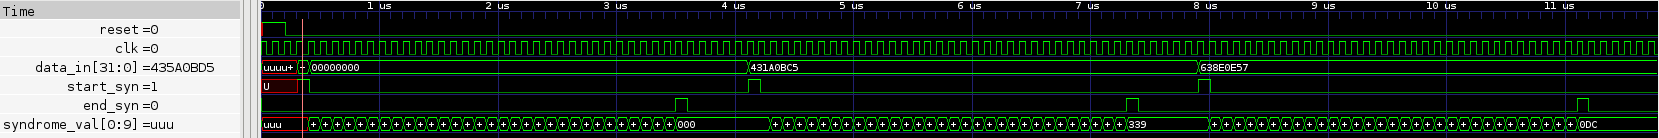
\includegraphics[width=\textwidth]{./images/syndrome_simu.png}
                \caption{Validation calcul du syndrome}
                \label{fig:sim_syndrome}
            \end{figure}

        \section{Look Up Table}
            \paragraph{}
                La Look Up Table n'a pas posé de problèmes d'implémentation. Le
                code VHDL de l'unité de traitement, de l'unité de contrôle et
                de l'assemblage est disponible en annexe \ref{ann:vhdl_lut}.

            \paragraph{}
                L'unité de traitement est composé d'un unique processus, sensible
                uniquement à l'horloge qui est chargé de la gestion P1 ou P2 en
                fonction des signaux venant de l'unité de contrôle.
                Elle possède aussi les sorties combinatoires suivantes~:
                \begin{itemize}
                    \item \verb|P1_MAX| indiquant si le pointeur 1 a atteint sa valeur maximale
                    \item \verb|P2_MAX| indiquant si le pointeur 2 a atteint sa valeur maximale
                    \item \verb|ERR1| indiquant si une seule erreur a été détectée
                    \item \verb|ERR2| indiquant si deux erreurs ont été détectées
                \end{itemize}

            \paragraph{}
                Le contrôle de P1 et de P2 se fait via les signaux internes suivants~:
                \begin{itemize}
                    \item \verb|INC_P1| pour incrémenter P1
                    \item \verb|INC_P2| pour incrémenter P2
                    \item \verb|RAZ| pour remettre à 0 P1 et P2 à 1
                    \item \verb|LD_P2| pour mettre P2 à la valeur de P1 courante
                \end{itemize}

            \paragraph{}
                La validation de la Look Up Table est faite à partir de
                syndromes calculés selon le tableau dans le sujet. Par exemple,
                pour le syndrome \verb|0000110010|, on vérifie que l'on obtient
                bien 2 erreurs, aux positions 15 et 18. Le même genre de test
                est effectué pour les cas extrêmes. Ce cas et les signaux
                intéressants sont présentés en figure~\ref{fig:sim_lut}.

                \begin{figure}[H]
                    \centering
                    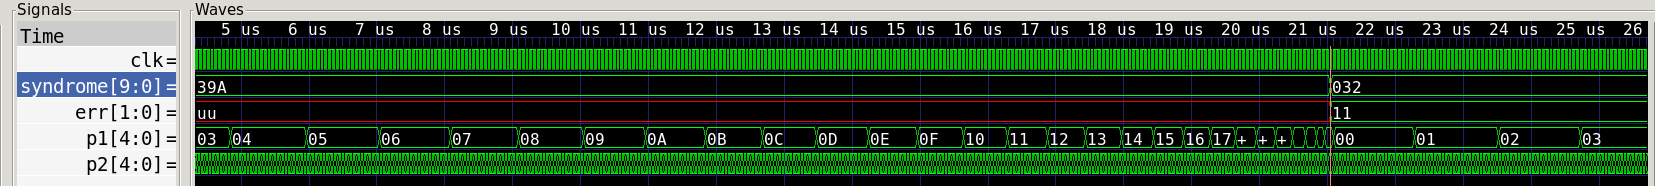
\includegraphics[width=\textwidth]{./images/lut_simu}
                    \caption{Validation LUT}
                    \label{fig:sim_lut}
                \end{figure}

        \section{Correcteur}
            \paragraph{}
                Le développement du correcteur n'a pas posé de problèmes
                particuliers. Les codes VHDL de l'unité de traitement, de
                l'unité de contrôle et l'assemblage sont disponibles en
                annexe~\ref{ann:vhdl_correcteur}.

            \paragraph{}
                L'unité de traitement est composée d'un unique processus,
                uniquement sensible à l'horloge. Il se charge du compteur
                interne ainsi que des divers signaux de chargement et de
                décalage provenant de l'unité de contrôle.
                Elle possède aussi deux sorties combinatoires~:
                 \begin{itemize}
                    \item \verb|D_CORR_OUT| pour rendre le résultat final de la
                        correction du message disponible dans le système principal.
                    \item \verb|CPT| pour que l'unité de contrôle ait en temps
                        réel l'état du compteur afin de prendre les décisions.
                \end{itemize}

            \paragraph{}
                Le contrôle des registres de décalage et de recomposition
                s'effectue grâce aux signaux suivants~:
                 \begin{itemize}
                    \item \verb|DEC_BUF| pour que le registre contenant le
                        message à traiter réalise un décalage de 1 bit vers la
                         droite, soit du MSB vers le LSB.
                    \item \verb|LD_BUF| pour charger un nouveau message dans le
                        registre de décalage.
                    \item \verb|LD_CORR| pour charger un nouveau bit dans le
                        registre recomposant le message corrigé.
                \end{itemize}

            \paragraph{}
                La validation du correcteur s'effectue en donnant le message de
                l'exemple, sans erreur, et en lui modifiant d'abord un, puis
                plusieurs bits. On s'attend ensuite à récupérer le message de
                l'exemple, donc corrigé par le module. On peut vérifier ce
                fonctionnement pour une et deux erreurs. Dans le cas ou il n'y
                a pas d'erreurs, le message n'est bien évidemment pas modifié.
                Lorsque plus de 2 erreurs sont présentes, le message est
                corrigé, mais en un autre message, plus proche statistiquement
                que le message d'origine. Le fonctionnement de l'implémentation
                VHDL est prouvé par les figures~\ref{fig:sim_corr_0},
                \ref{fig:sim_corr_1}, \ref{fig:sim_corr_2},
                \ref{fig:sim_corr_3} ci-dessous.

                \begin{figure}[H]
                    \centering
                    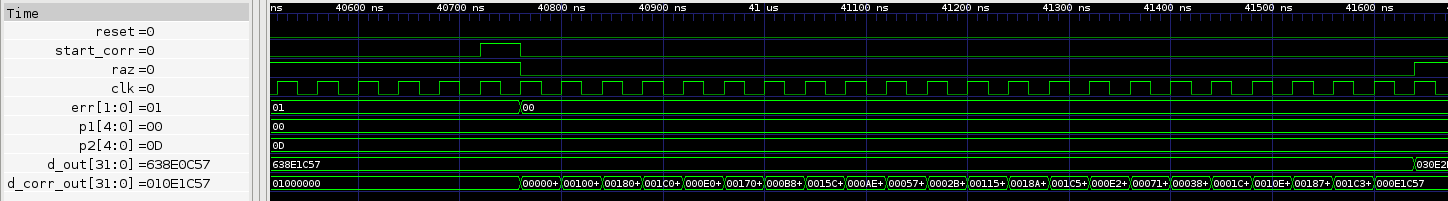
\includegraphics[width=\textwidth]{./images/corr_0_err.png}
                    \caption{Effet de la correction lorsqu'il n'y a pas d'erreurs.}
                    \label{fig:sim_corr_0}
                \end{figure}

                \begin{figure}[H]
                    \centering
                    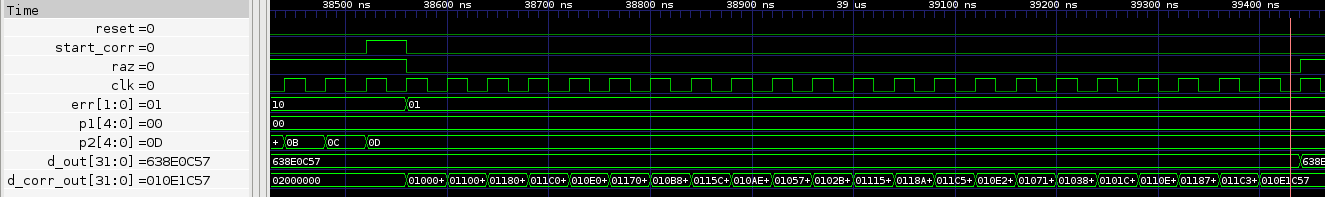
\includegraphics[width=\textwidth]{./images/corr_1_err.png}
                    \caption{Correction d'une erreur.}
                    \label{fig:sim_corr_1}
                \end{figure}

                \begin{figure}[H]
                    \centering
                    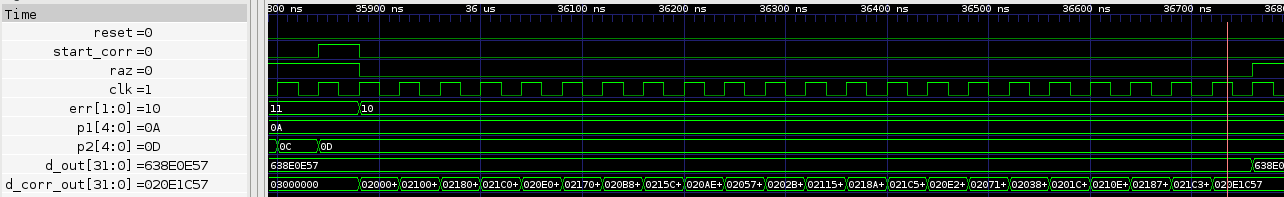
\includegraphics[width=\textwidth]{./images/corr_2_err.png}
                    \caption{Correction de deux erreurs.}
                    \label{fig:sim_corr_2}
                \end{figure}

                \begin{figure}[H]
                    \centering
                    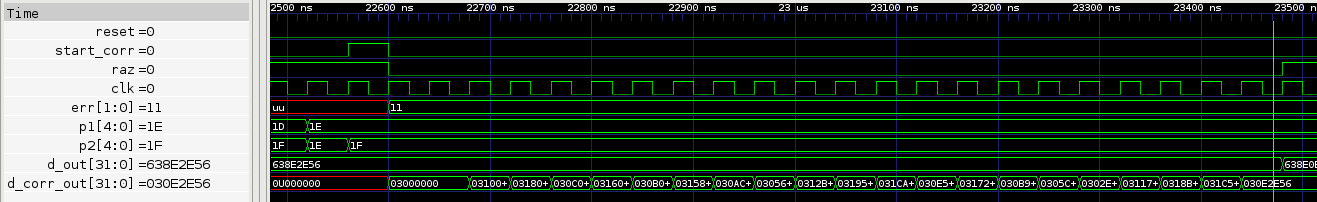
\includegraphics[width=\textwidth]{./images/corr_2sup_err.png}
                    \caption{Absence de correction pour plus de deux erreurs.}
                    \label{fig:sim_corr_3}
                \end{figure}

        \section{Interface Avalon}
            \paragraph{}
                L'interface avalon permet de s'interfacer avec le processeur. Cette
                partie n'a pas posé de problème particulier. Le code est disponible en annexe
                \ref{ann:vdhl_avalon}

            \paragraph{}
                L'interface avalon est composée d'un processus réagissant à
                l'horloge ainsi qu'a un signal reset.  Ce processus permet de
                gérer les écritures sur les coups d'horloge.  Elle possède
                aussi plusieurs sorties combinatoires destinées à la sortie
                vers le processeur, au contrôle de la FIFO et aux
                interruptions.

            \paragraph{}
                Afin de vérifier le fonctionnement de l'interface, nous avons
                écrit un test pour tester l'écriture et la lecture de tous les
                registres ainsi que les interruptions. La figure
                \ref{fig:sim_avalon} montre l'écriture dans la pile depuis
                l'interface avalon.

                \begin{figure}[H]
                    \centering
                    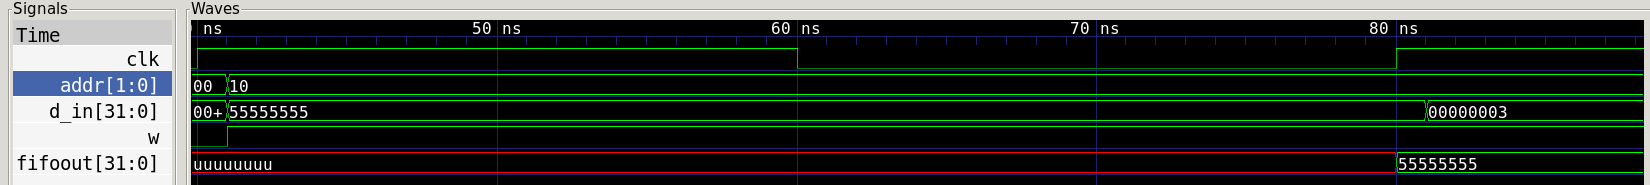
\includegraphics[width=\textwidth]{./images/avalon_simu}
                    \caption{Validation avalon}
                    \label{fig:sim_avalon}
                \end{figure}

        \section{Assemblage des briques}
            \paragraph{}
                Une fois toutes les briques crées, il faut les assembler et les
                piloter. Là encore, pas de soucis majeurs, il s'agit d'un
                simple câblage et d'une machine à états maitre.  Le code source
                de l'assemblage est disponible en annexe \ref{ann:vhdl_bch} et
                celui de la machine à états maitre en annexe \ref{ann:vhdl_master}.

            \paragraph{}
                La machine à états maitre permet de piloter tous les blocs de notre décodeur.
                Pour la tester, nous avons juste envoyé le signal start puis
                envoyé les signaux de fin de fonctionnement de chaque bloc,
                dans l'ordre. Nous avons aussi testé avec un syndrome nul pour vérifier
                que dans ce cas, la Look Up Table était bien ignorée.
                Le résultat de ce test peut être vu en figure \ref{fig:sim_master}
                \begin{figure}[H]
                    \centering
                    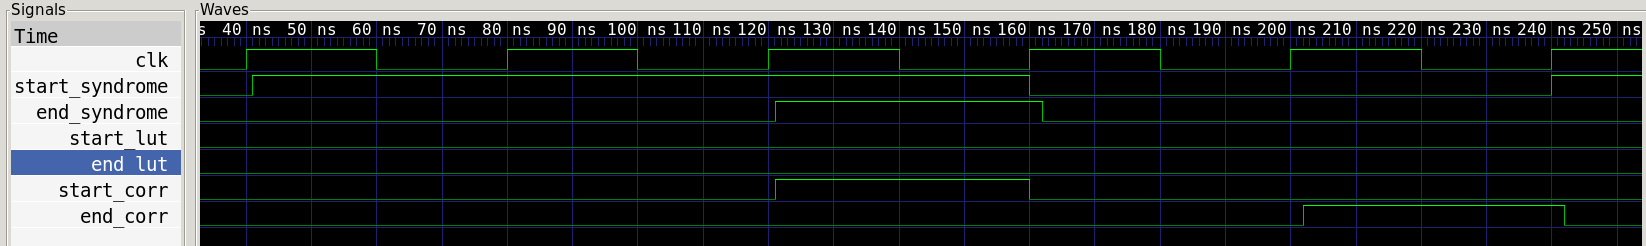
\includegraphics[width=\textwidth]{./images/master_simu}
                    \caption{Validation machine à états maitre}
                    \label{fig:sim_master}
                \end{figure}

            \paragraph{}
                La validation de l'assemblage complet est fait par une
                simulation de notre programme de test en forçant les signaux à
                la main.  On envoie des messages avec 3, 2, 1 et 0 erreurs et
                on vérifie qu'on obtient bien une interruption et le message
                corrigé si possible.  La vérification est visible en figure
                \ref{fig:sim_bch}

                \begin{figure}[H]
                    \centering
                    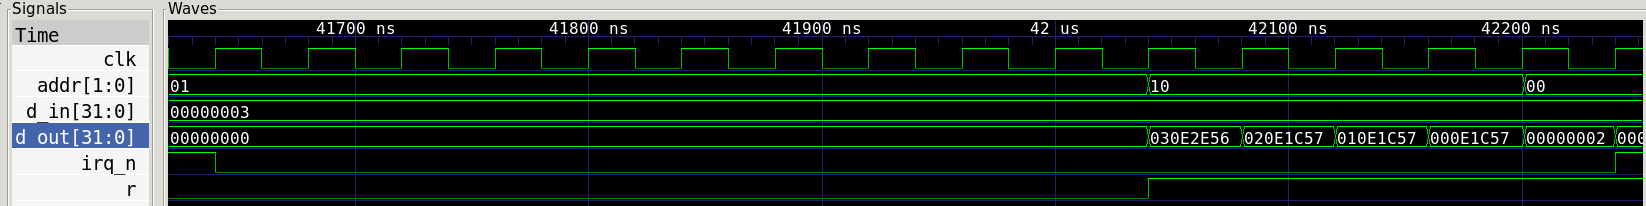
\includegraphics[width=\textwidth]{./images/bch_simu}
                    \caption{Validation de l'assemblage}
                    \label{fig:sim_bch}
                \end{figure}

    \chapter{Spécification du composant librairie}
        \paragraph{}
            Les différentes figures qui suivent, décrivent les diverses
            parties du composant de librairie issu du code vhdl. On pourra y
            voir les caractéristiques et les connexions des différents signaux
            notables du module BCH que nous avons créé.

        \begin{figure}[H]
            \centering
            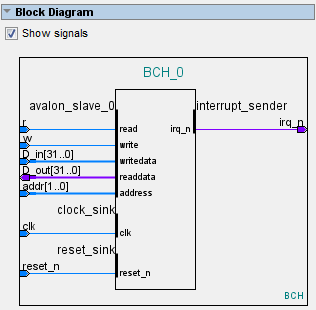
\includegraphics[width=\textwidth]{./images/BCH_0_block_diagram}
            \caption{Diagramme bloc du BCH et ses signaux}
            \label{fig:BCH_0_block_diagram}
        \end{figure}

        \begin{figure}[H]
            \centering
            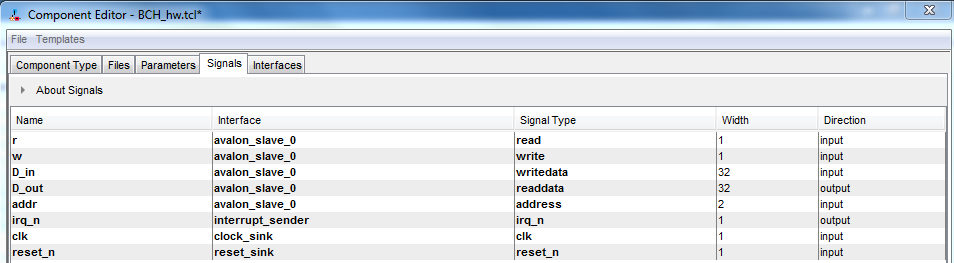
\includegraphics[width=\textwidth]{./images/BCH_hw_signals}
            \caption{Connexions et caractéristiques des signaux du module BCH}
            \label{fig:BCH_hw_signals}
        \end{figure}

        \begin{figure}[H]
            \centering
            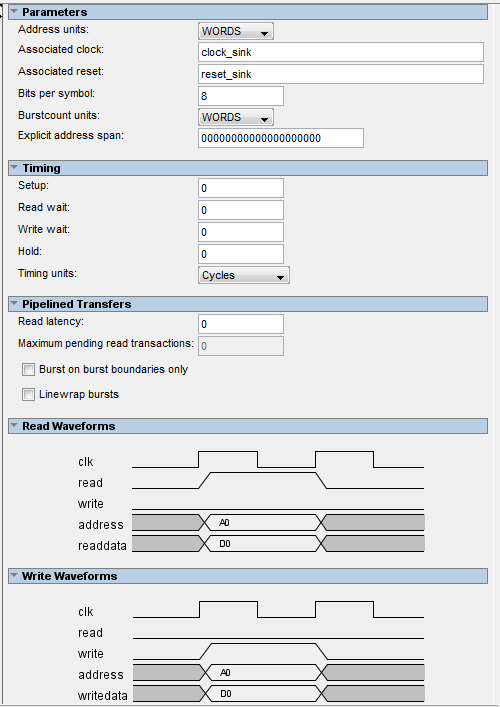
\includegraphics[width=\textwidth]{./images/BCH_0_parameters}
            \caption{Paramètres de synthèse du composant BCH}
            \label{fig:BCH_0_parameters}
        \end{figure}

        \begin{figure}[H]
            \centering
            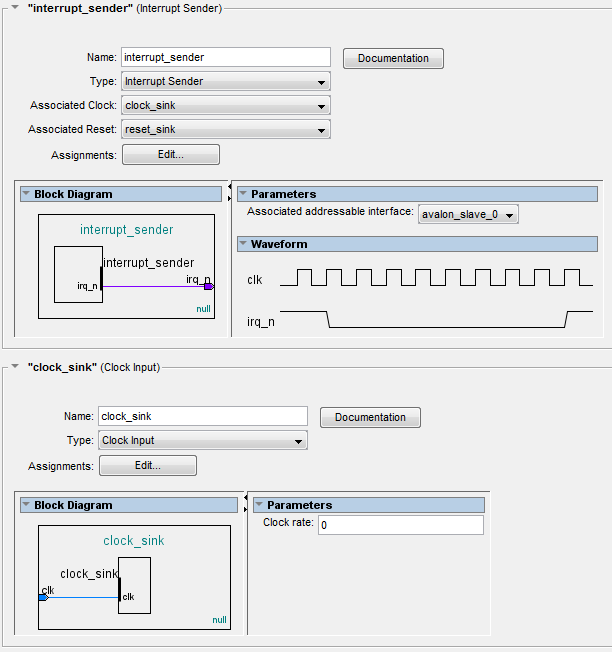
\includegraphics[width=\textwidth]{./images/interrupt_sender}
            \caption{Paramètres du gestionnaire d'interruptions du BCH}
            \label{fig:interrupt_sender}
        \end{figure}

        \begin{figure}[H]
            \centering
            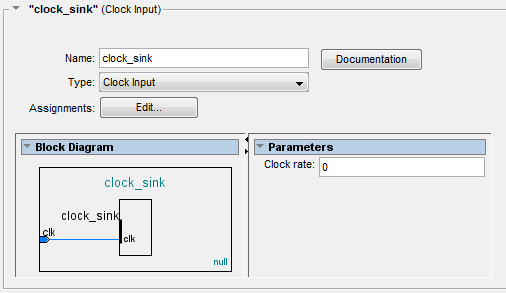
\includegraphics[width=\textwidth]{./images/clock_sink}
            \caption{Paramètres du signal d'horloge connecté au BCH}
            \label{fig:clock_sink}
        \end{figure}

        \begin{figure}[H]
            \centering
            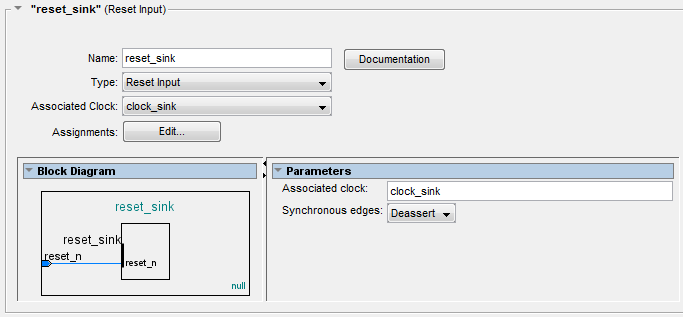
\includegraphics[width=\textwidth]{./images/reset_sink}
            \caption{Paramètres du signal de reset connecté au BCH}
            \label{fig:reset_sink}
        \end{figure}

    \chapter{Synthèse logique et simulation structurelle}
        \paragraph{}
        La figure ~\ref{fig:BCH_0_component} montre le composant $BCH_0$, dans
        la liste des composants synthétisés qui seront chargés sur le FPGA.

        \begin{figure}[H]
            \centering
            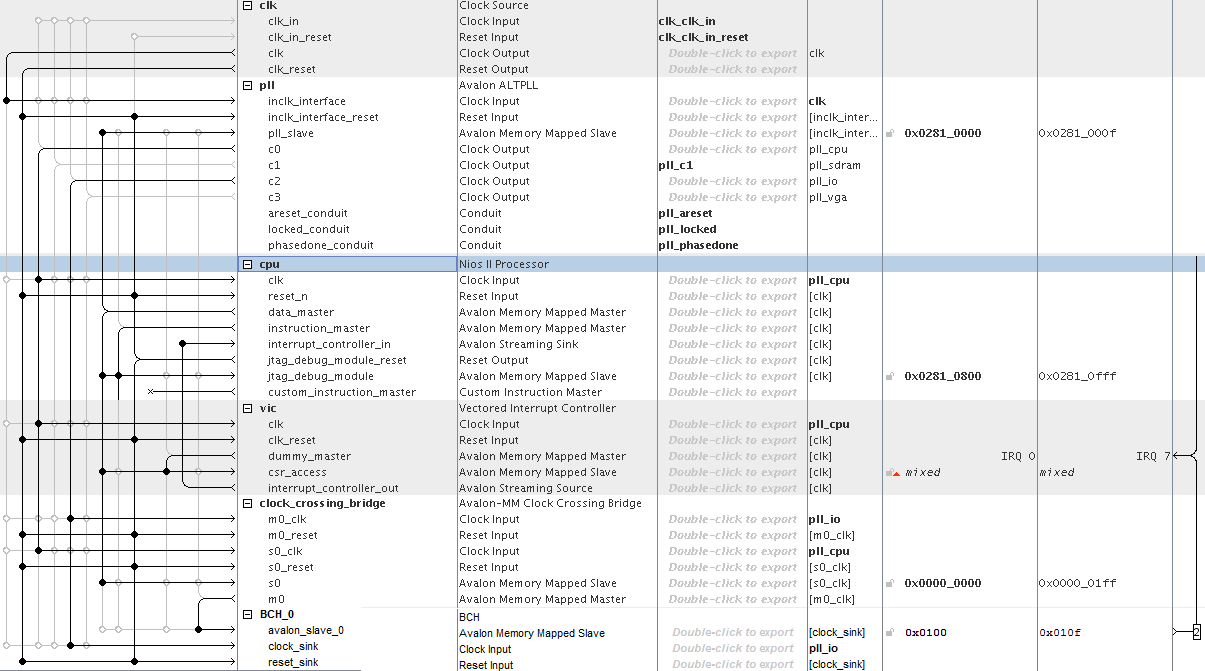
\includegraphics[width=\textwidth]{./images/BCH_0_component}
            \caption{Composant BCH ajouté aux modules du processeur}
            \label{fig:BCH_0_component}
        \end{figure}

        \paragraph{}
        La compilation du projet avec le composant BCH nous à d'abord révélé
        des erreurs simples dans le code VHDL qui aboutissaient à la création
        de Latch. Après vérification et relecture du code les soucis venaient
        d'oublis du signal d'horloge dans la liste de sensibilités de certains
        processus.

        \paragraph{}
        La simulation structurelle montre que notre implémentation
        du BCH est viable et conforme au cahier des charges.

    \chapter{Présentation de l'API c}

    Maintenant que le composant est implémenté et que le projet quartus est
    compilé et flashé il est nécessaire d'implémenter une api permettant
    d'utiliser le composant de façon assez confortable. L'api que nous
    proposons est assez riche.

    \section{Structure de donnée}

    Inclue en annexe~\ref{ann:api_h}, nous avons écrit une structure qui permet
    de récupérer une paire, message et erreur. Le message présent dans la
    structure est le message corrigé si possible et le champ erreur permet de
    connaitre le nombre d'erreurs détectés.

    \section{Définition de l'API}

    L'api est définie en annexe~\ref{ann:api_h} mais est présentée plus en
    détail dans les sections suivantes.

    \subsection{Envoi et récupération de messages}

    Deux fonctions permettent l'échange de message à corriger et corrigé. Il
    s'agit de \verb$BCH_push_msg$ et \verb$BCH_pop_msg$. La première envoie un
    message à corriger sous forme d'entier non signé et la seconde récupère un
    message corrigé sous forme de structure \verb$bch_msg$.

    \subsection{Lecture du registre de statu}

    La lecture du statu ce fait avec la fonction \verb$BCH_read_status$ qui
    renvoi la valeur non signé présente sur le bus de statu. L'utilisateur à
    alors la responsabilité d'utiliser les opérateurs logiques «~et~» et «~ou~»
    afin de récupérer la valeur qui l'intéresse dans le statu. Si une seule
    valeur l'intéresse, ou que le cout de lecture répété d'un registre n'est
    pas dérangeant l'utilisateur dispose de fonctions raccourcis pui permettent
    d'accéder à une information ciblée du statu~:
    \begin{itemize}
        \item \verb$BCH_is_full$ nous donne si la pile est pleine
        \item \verb$BCH_is_empty$ nous donne si la pile est vide ou non
        \item \verb$BCH_is_irq$ nous donne si le traitement est terminé
    \end{itemize}

    \subsection{Lecture et écriture du registre de contrôle}

    De la même manière que pour le registre de statu l'utilisateur dispose des
    fonctions \verb$BCH_read_ctrl$ et de \verb$BCH_write_ctrl$. Et de même il
    peut utiliser des fonctions raccourcis pour lire et changer des valeurs sans
    avoir à manipuler manuellement le registre de contrôle. Les fonctions sont
    les suivantes~:
    \begin{itemize}
        \item \verb$BCH_is_irq_enabled$ qui permet de savoir si les irq sont activé ou non
        \item \verb$BCH_is_decoding$ qui permet de savoir si le décodeur est en marche
        \item \verb$BCH_ack_irq$ qui permet de désarmer une interruption
        \item \verb$BCH_enable_irq$ qui permet d'activer les interruptions
        \item \verb$BCH_isable_irq$ qui permet de désactiver les interruptions
        \item \verb$BCH_start$ qui permet de lancer le décodage
    \end{itemize}


    \chapter{Application de démonstration}

        \paragraph{}
        Dans le code applicatif présenté en annexe~\ref{ann:demo}, nous
        réalisons un test de fonctionnement des demandes d'interruptions et
        d'appel de la routine d'interruption, si celle-ci a été préalablement
        autorisée. Nous envoyons deux séries de 4 messages, chacune allant
        progressivement de 0 erreur pour le premier message, à trois erreurs
        pour le quatrième. Dans les trois premiers cas, on s'attend à ce qu'au
        final, le bon message soit récupéré. Le dernier cependant, comportant
        trois erreurs, ne sera pas corrigé. Cela est due au fait que ce modèle
        de BCH ne peut corriger que deux erreurs au maximum, et en détecter
        jusqu'à cinq.

        \paragraph{}
        La première série de messages est donc donnée au BCH, qui une fois les
        interruptions autorisées, commencera à les traiter. Lorsque tous les
        messages ont été corrigés, le drapeau de demande d'interruption va se
        lever. Les interruptions étant activées, la routine sera lancée et
        videra la pile en nous faisant part des résultats.

        \paragraph{}
        La deuxième série de messages, identique à la première, sera passée au
        BCH, mais cette fois-ci, les demandes d'interruptions seront
        désactivées. Lorsque le BCH aura terminé le traitement des messages,
        le drapeau de demande d'interruption se lèvera bien de nouveau, mais
        la routine d'interruption ne sera pas déclenchée. C'est donc bien le
        fonctionnement souhaité qui est réalisé. Afin d'être certain que les
        messages ont cependant bien été traités, à la suite de la levée du
        drapeau de demande d'interruption du BCH, nous venons vider la pile
        en faisant à nouveau part des résultats. Résultats qui sont bien les
        mêmes que précédemment.

        \paragraph{}
        Le code applicatif présenté précédemment génère les sorties suivantes dans la console~:

        \paragraph{}
        \begin{minted}[linenos]{text}
        Hello from Nios II!
        Status: 0x3
        Control: 0x0
        Status: 0x1
        Status: 0x1
        Status: 0x1
        Status 1: 0x5
        Control 1: 0x2
        Status 2: 0x5
        Error 1: 0x0, Data: 0x1A0BD5; Status: 0x0; Ctrl: 0x2
        Error 2: 0x1, Data: 0x1A0BD5; Status: 0x1; Ctrl: 0x2
        Error 3: 0x2, Data: 0x1A0BD5; Status: 0x1; Ctrl: 0x2
        Error 4: 0x3, Data: 0x1A1AD4; Status: 0x3; Ctrl: 0x2
        Status 3: 0x3
        First pass with irqs enabled done!
        Status: 0x1
        Status: 0x1
        Status: 0x1
        Status: 0x5
        Control: 0x0
        Second pass with irqs disabled done! irq_n=0 but no ISR called
        Control: 0x0
        Status: 0x5
        Error: 0x0, Data: 0x1A0BD5; Status: 0x1; Ctrl: 0x0
        Error: 0x1, Data: 0x1A0BD5; Status: 0x1; Ctrl: 0x0
        Error: 0x2, Data: 0x1A0BD5; Status: 0x1; Ctrl: 0x0
        Error: 0x3, Data: 0x1A1AD4; Status: 0x3; Ctrl: 0x0
        \end{minted}


        \begin{figure}[H]
            \centering
            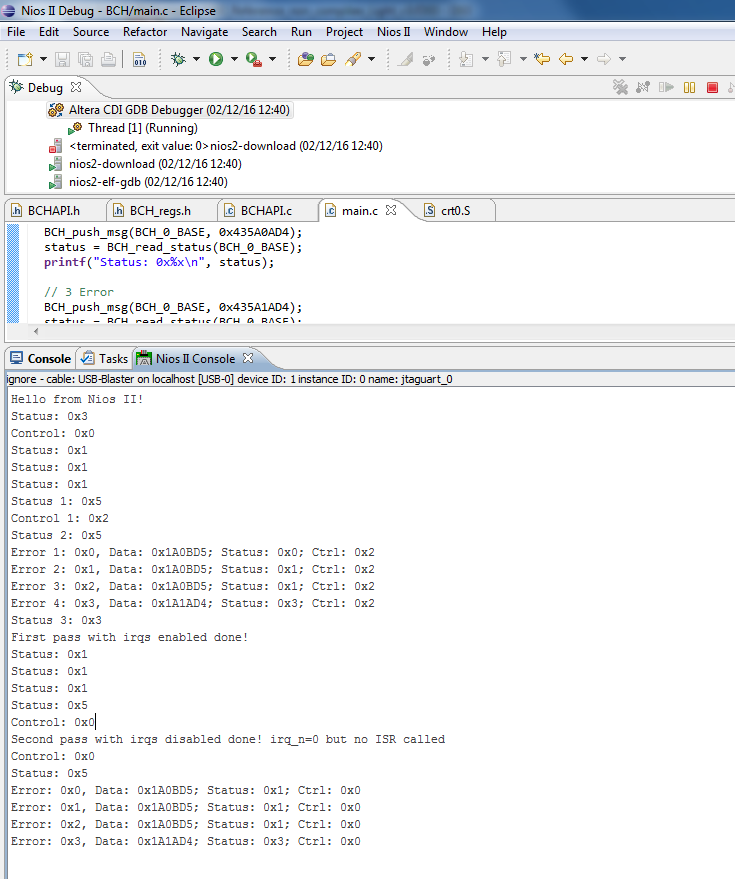
\includegraphics[width=\textwidth]{./images/bch_output}
            \caption{Sortie générée par le BCH dans la console Eclipse}
            \label{fig:bch_output}
        \end{figure}

    \begin{appendices}

        \chapter{Code VHDL}

        \section{Calcul du syndrome}
        \label{ann:vhdl_syndrome}
        \subsection{Unité de traitement}
        \inputminted[firstline=0, lastline=51,breaklines]{VHDL}{../src/ut_syndrome.vhd}
        \subsection{Unité de contrôle}
        \inputminted[firstline=0, lastline=81,breaklines]{VHDL}{../src/uc_syndrome.vhd}
        \subsection{Assemblage UT/UC}
        \inputminted[firstline=0, lastline=44,breaklines]{VHDL}{../src/syndrome.vhd}

        \section{Look up table}
        \label{ann:vhdl_lut}
        \subsection{Unité de traitement}
        \inputminted[firstline=0, lastline=84,breaklines]{VHDL}{../src/ut_lut.vhd}
        \subsection{Unité de contrôle}
        \inputminted[firstline=0, lastline=72,breaklines]{VHDL}{../src/uc_lut.vhd}
        \subsection{Assemblage UT/UC}
        \inputminted[firstline=0, lastline=90,breaklines]{VHDL}{../src/lut.vhd}

        \section{Correcteur}
        \label{ann:vhdl_correcteur}
        \subsection{Unité de traitement}
        \inputminted[firstline=0, lastline=61,breaklines]{VHDL}{../src/ut_corr.vhd}
        \subsection{Unité de contrôle}
        \inputminted[firstline=0, lastline=53,breaklines]{VHDL}{../src/uc_corr.vhd}
        \subsection{Assemblage UT/UC}
        \inputminted[firstline=0, lastline=45,breaklines]{VHDL}{../src/corr.vhd}

        \section{Fifo}
        La pile fifo utilisée est celle proposé sur l'Ent.
        \inputminted[firstline=0, lastline=65,breaklines]{VHDL}{../src/fifo.vhd}

        \section{Interface Avalon}
        \label{ann:vhdl_avalon}
        \inputminted[firstline=0, lastline=86,breaklines]{VHDL}{../src/avalon.vhd}

        \section{Unité de contrôle maitre}
        \label{ann:vhdl_master}
        \inputminted[firstline=0, lastline=90,breaklines]{VHDL}{../src/uc_master.vhd}

        \section{Décodeur BCH complet}
        \label{ann:vhdl_bch}
        \inputminted[firstline=0, lastline=113,breaklines]{VHDL}{../src/bch.vhd}

        \chapter{Drivers et API}

        \section{Définition des registres}
        \inputminted[breaklines]{C}{../quartus/ip/BCH/inc/BCH_regs.h}

        \section{API}
        \subsection{Headers}
        \label{ann:api_h}
        \inputminted[breaklines]{C}{../quartus/ip/BCH/inc/BCHAPI.h}
        \subsection{Sources}
        \inputminted[breaklines]{C}{../quartus/ip/BCH/src/BCHAPI.c}

        \chapter{Code applicatif de démonstration}
        \label{ann:demo}
        \inputminted[breaklines]{C}{../quartus/software/BCH/main.c}


    \end{appendices}

\end{document}
